% =====================================================================
%  Slide bảo vệ khóa luận tốt nghiệp
%  "Nghiên cứu phương pháp xây dựng NeoBERT cho tiếng Việt"
%  Biên dịch:  latexmk -pdf main.tex     (hoặc: make)
% =====================================================================
\documentclass[aspectratio=169,10pt,t]{beamer}   % t = nội dung bám mép trên

\usepackage[utf8]{inputenc}
\usepackage[T5]{fontenc}
\usepackage[vietnamese]{babel}
\usepackage{graphicx}
\usepackage{amsmath,amssymb}
\usepackage{array}
\usepackage[authoryear,square]{natbib}

\usepackage{vineo-theme}

\usetikzlibrary{arrows.meta,positioning,calc,fit,backgrounds,shapes.geometric,
                decorations.pathreplacing}

\setbeamertemplate{bibliography item}[triangle]
\graphicspath{{figures/}}

% ------------------------------------------------------------------ metadata
\title[Khóa luận tốt nghiệp]{Nghiên cứu phương pháp xây dựng\\NeoBERT cho tiếng Việt}
\author[Trung -- Tú]{Bùi Khắc Trung \and Trần Anh Tú}
\institute[HCMUS]{Khoa Công nghệ Thông tin, Trường ĐH Khoa học Tự nhiên, ĐHQG-HCM}
\date[Tháng 07/2026]{Tp. Hồ Chí Minh, tháng 07 năm 2026}

\begin{document}

% ------------------------------------------------------------------ bìa
\begin{frame}[plain]
  \centering
  \vspace{0.2em}
  {\footnotesize\color{vnNavy}
   TRƯỜNG ĐẠI HỌC KHOA HỌC TỰ NHIÊN, ĐHQG-HCM\\
   KHOA CÔNG NGHỆ THÔNG TIN\par}

  \vspace{0.5em}
  
\includegraphics[width=1.35cm]{logo-hcmus}

  \vspace{0.4em}
  {\footnotesize\bfseries\color{vnSteel} KHÓA LUẬN TỐT NGHIỆP\par}

  \vspace{0.5em}
  {\color{vnSteel!45}\rule{0.72\textwidth}{0.8pt}\par}
  \vspace{0.4em}
  {\large\bfseries\color{vnNavy}
   NGHIÊN CỨU PHƯƠNG PHÁP XÂY DỰNG\\[2pt]
   NEOBERT CHO TIẾNG VIỆT\par}
  \vspace{0.4em}
  {\color{vnSteel!45}\rule{0.72\textwidth}{0.8pt}\par}

  \vspace{0.9em}
  % Ba cột: hướng dẫn -- phản biện -- sinh viên. Mỗi khe giữa hai cột tốn
  % ~0.42cm, nên tổng bề rộng cột phải dưới 0.94\textwidth.
  \begin{columns}[t]
    \begin{column}{0.30\textwidth}\centering\footnotesize
      {\bfseries\color{vnNavy} Giảng viên hướng dẫn}\\[3pt]
      TS. Nguyễn Hồng Bửu Long\\
      TS. Lương An Vinh
    \end{column}
    \begin{column}{0.30\textwidth}\centering\footnotesize
      {\bfseries\color{vnNavy} Giảng viên phản biện}\\[3pt]
      ThS. Trần Thị Thảo Nhi
    \end{column}
    \begin{column}{0.30\textwidth}\centering\footnotesize
      {\bfseries\color{vnNavy} Sinh viên thực hiện}\\[3pt]
      Bùi Khắc Trung -- 22120396\\
      Trần Anh Tú -- 22120400
    \end{column}
  \end{columns}

  \vfill
  {\scriptsize\color{vnCite} Tp. Hồ Chí Minh, tháng 07 năm 2026\par}
  \vspace{0.3em}
\end{frame}

% ------------------------------------------------------------------ mục lục
\begin{frame}{Nội dung trình bày}
  \vspace{0.6em}
  \begin{columns}[T]
    \begin{column}{0.62\textwidth}
      \tableofcontents[subsectionstyle=show/show]
    \end{column}
    \begin{column}{0.34\textwidth}
      \small
      \begin{block}{Câu hỏi của khóa luận}
        Làm sao chuyển một mô hình Encoder thế hệ mới sang tiếng Việt
        \emph{mà không} huấn luyện lại từ đầu?
      \end{block}
    \end{column}
  \end{columns}
\end{frame}

% =====================================================================
\section{Giới thiệu}
% =====================================================================

% ---------------------------------------------------------------------
\begin{frame}{Encoder-only: nền tảng của các bài toán hiểu ngôn ngữ}
\vspace{0.2em}
\begin{columns}[T]
\begin{column}{0.54\textwidth}
  \textbf{Encoder-only là gì?}
  \begin{itemize}\itemsep3pt
    \item Đọc câu theo \emph{cả hai chiều}, sinh ra biểu diễn ngữ nghĩa
          cho từng từ -- không sinh văn bản.
    \item Là lựa chọn mặc định cho phân loại văn bản, gán nhãn, hỏi đáp
          trích xuất, tìm kiếm ngữ nghĩa.
    \item BERT và RoBERTa vẫn đang được dùng rộng rãi trong thực tế.
  \end{itemize}
\end{column}

\begin{column}{0.43\textwidth}
  \begin{block}{Vấn đề}
    Trong khi các mô hình sinh văn bản (LLM) tiến hóa liên tục, các mô
    hình dòng Encoder-only đã \emph{chững lại nhiều năm}, chỉ được cập
    nhật tiếp từ cuối năm 2024.
  \end{block}
\end{column}
\end{columns}

\vspace{0.5em}
\centering
% Mốc thời gian hai dòng mô hình. Trục hoành: 1 đơn vị = 1 năm, gốc = 01/2018,
% vị trí mốc tính theo tháng phát hành thực tế. Nhãn xếp so le hai tầng để các
% mốc gần nhau không đè lên nhau. Dòng Encoder dùng nét đứt cho quãng 2021-2024.
\fitpic{\begin{tikzpicture}[font=\tiny,x=1.62cm,y=1.32cm]

  % ---- dòng mô hình sinh văn bản: nhiều nhóm nghiên cứu, năm nào cũng có mốc
  \node[anchor=east,text=vnSteel,font=\scriptsize\bfseries] at (-0.3,0.72) {LLM};
  \draw[vnSteel,thick,-{Latex[length=2mm]}] (-0.2,0.72) -- (7.55,0.72);
  % tầng gần trục
  \foreach \x/\lb in {0.42/GPT-1, 2.33/GPT-3, 4.25/PaLM, 5.20/GPT-4}{
    \fill[vnSteel] (\x,0.72) circle (1.4pt);
    \node[above=1pt,text=vnSteel] at (\x,0.72) {\lb};
  }
  % tầng xa trục
  \foreach \x/\lb in {1.08/GPT-2, 3.94/Gopher, 4.87/ChatGPT, 6.25/{Llama 3},
                      7.05/{DeepSeek-R1}}{
    \fill[vnSteel] (\x,0.72) circle (1.4pt);
    \draw[vnSteel!45,line width=0.3pt] (\x,0.72) -- (\x,0.94);
    \node[above=0pt,text=vnSteel] at (\x,0.94) {\lb};
  }

  % ---- trục năm ở giữa
  \foreach \x/\yr in {0/2018,1/2019,2/2020,3/2021,4/2022,5/2023,6/2024,7/2025}{
    \node[text=vnInk!65] at (\x,0.30) {\yr};
  }

  % ---- dòng Encoder: liền nét -> đứt quãng -> liền nét trở lại
  \node[anchor=east,text=vnNavy,font=\scriptsize\bfseries] at (-0.3,-0.02) {Encoder};
  \draw[vnNavy,thick]        (-0.2,-0.02) -- (3.88,-0.02);
  \draw[vnNavy,thick,dashed] (3.88,-0.02) -- (6.80,-0.02);
  \draw[vnNavy,thick,-{Latex[length=2mm]}] (6.80,-0.02) -- (7.55,-0.02);
  % tầng gần trục
  \foreach \x/\lb in {0.78/BERT, 2.42/DeBERTa}{
    \fill[vnNavy] (\x,-0.02) circle (1.4pt);
    \node[below=1pt,text=vnNavy] at (\x,-0.02) {\lb};
  }
  % tầng xa trục
  \foreach \x/\lb in {1.56/RoBERTa, 3.88/{DeBERTaV3}}{
    \fill[vnNavy] (\x,-0.02) circle (1.4pt);
    \draw[vnNavy!45,line width=0.3pt] (\x,-0.02) -- (\x,-0.24);
    \node[below=0pt,text=vnNavy] at (\x,-0.24) {\lb};
  }
  % ---- đợt hiện đại hóa: hai mốc chỉ cách nhau 2 tháng nên nhãn phải tách ra,
  %      ModernBERT lùi hẳn sang trái, NeoBERT xuống tầng dưới cùng.
  \fill[vnNavy] (6.92,-0.02) circle (1.4pt);
  \draw[vnNavy!45,line width=0.3pt] (6.92,-0.02) -- (6.66,-0.16);
  \node[anchor=north east,text=vnNavy,align=right] at (6.64,-0.17) {ModernBERT\\12/2024};
  \fill[vnRed] (7.08,-0.02) circle (2.2pt);
  \draw[vnRed!45,line width=0.3pt] (7.08,-0.02) -- (7.08,-0.42);
  \node[below=0pt,text=vnRed,font=\tiny\bfseries,align=center] at (7.08,-0.42)
       {NeoBERT\\02/2025};
\end{tikzpicture}}
\end{frame}

% ---------------------------------------------------------------------
\begin{frame}{NeoBERT (2025) hiện đại hóa Encoder -- nhưng chỉ có tiếng Anh}
\vspace{0.3em}
\begin{columns}[T]
\begin{column}{0.52\textwidth}
  \textbf{NeoBERT} \cit{LeBreton2025} đưa các cải tiến của thế hệ LLM
  trở lại kiến trúc Encoder:
  \begin{itemize}\itemsep2pt
    \item \textbf{RoPE} -- mã hóa vị trí bằng phép quay
    \item \textbf{SwiGLU} -- mạng truyền thẳng có cổng
    \item \textbf{Pre-RMSNorm} -- chuẩn hóa trước mỗi lớp con
    \item \textbf{Sâu mà hẹp} -- 28 lớp, kích thước ẩn 768
  \end{itemize}

  \vspace{0.4em}
  Chỉ \textbf{250 triệu tham số} nhưng vượt BERT\textsubscript{large} và
  RoBERTa\textsubscript{large} trên chuẩn đánh giá MTEB, đồng thời hỗ trợ
  ngữ cảnh \textbf{4.096 token} -- gấp 8 lần BERT.
\end{column}

\begin{column}{0.45\textwidth}
  \small
  \begin{tabular}{@{}l l@{}}
    \toprule
    \rowcolor{vnLight}\multicolumn{2}{@{}l@{}}{\bfseries\color{vnNavy} Cấu hình NeoBERT}\\
    \midrule
    Số lớp / kích thước ẩn & 28 / 768\\
    Tham số                & $\approx$ 250 triệu\\
    Mã hóa vị trí          & RoPE\\
    Kích hoạt FFN          & SwiGLU\\
    Chuẩn hóa              & Pre-RMSNorm\\
    Ngữ cảnh tối đa        & 4.096 token\\
    Dữ liệu tiền huấn luyện& 2,1 nghìn tỷ token\\
    Ngôn ngữ               & \hl{chỉ tiếng Anh}\\
    \bottomrule
  \end{tabular}
  \vspace{4pt}
  {\footnotesize\color{vnCite} Bảng cấu hình theo \citet{LeBreton2025}}
\end{column}
\end{columns}
\end{frame}

% ---------------------------------------------------------------------
\begin{frame}{Bài toán: đưa NeoBERT sang tiếng Việt với chi phí chấp nhận được}
\vspace{0.2em}
\begin{columns}[T]
\begin{column}{0.49\textwidth}
  \textbf{Ba trở ngại}
  \begin{enumerate}\itemsep2pt
    \item Encoder tiếng Việt hiện có (PhoBERT \cit{Nguyen2020},
          ViDeBERTa \cit{Tran2023}) dùng kiến trúc cũ, giới hạn 512 token.
    \item Huấn luyện lại từ đầu cần \textbf{2,1 nghìn tỷ token} --
          bất khả thi với nhóm nghiên cứu nhỏ.
    \item Thay lớp véc-tơ rồi huấn luyện tiếp một cách ngây thơ dễ gây
          \term{mất thông tin}{catastrophic forgetting}.
  \end{enumerate}
\end{column}

\begin{column}{0.49\textwidth}
  \textbf{Ý tưởng của khóa luận}

  \vspace{2pt}
  \begin{block}{Tái sử dụng thay vì huấn luyện lại}
    Giữ nguyên \emph{phần thân} NeoBERT đã học từ tiếng Anh; chỉ thay
    lớp từ vựng, và khởi tạo lớp mới bằng cách \emph{mượn} không gian
    ngữ nghĩa tiếng Việt sẵn có của ViDeBERTa.
  \end{block}

  \vspace{2pt}
  \textbf{Mục tiêu cụ thể}
  \begin{itemize}\itemsep1pt
    \item Xây dựng \textbf{ViNeoBERT} bằng kỹ thuật SALT \cit{Lee2025}
          có cải tiến.
    \item Chứng minh bằng thực nghiệm rằng cách này \emph{tiết kiệm hơn
          nhiều} so với huấn luyện lại.
  \end{itemize}
\end{column}
\end{columns}
\end{frame}

% =====================================================================
\section{Cơ sở lý thuyết}
% =====================================================================

% ---------------------------------------------------------------------
\begin{frame}{Kiến trúc NeoBERT}
\vspace{-0.35em}
\centering
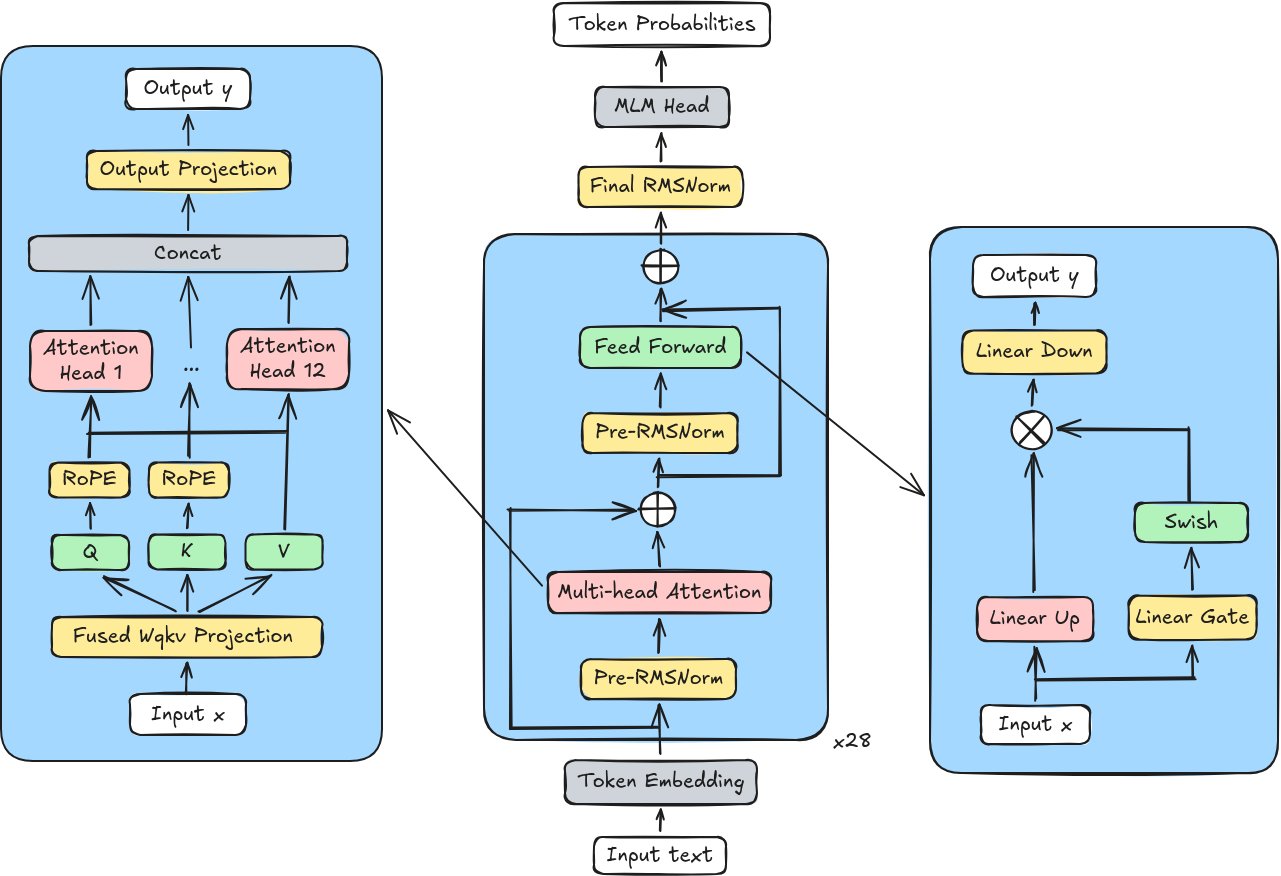
\includegraphics[width=\linewidth,height=7.05cm,keepaspectratio]{fig-neobert-arch}
\end{frame}

% ---------------------------------------------------------------------
\begin{frame}{RoPE: mã hóa vị trí bằng phép quay véc-tơ}
\vspace{0.2em}
\centering
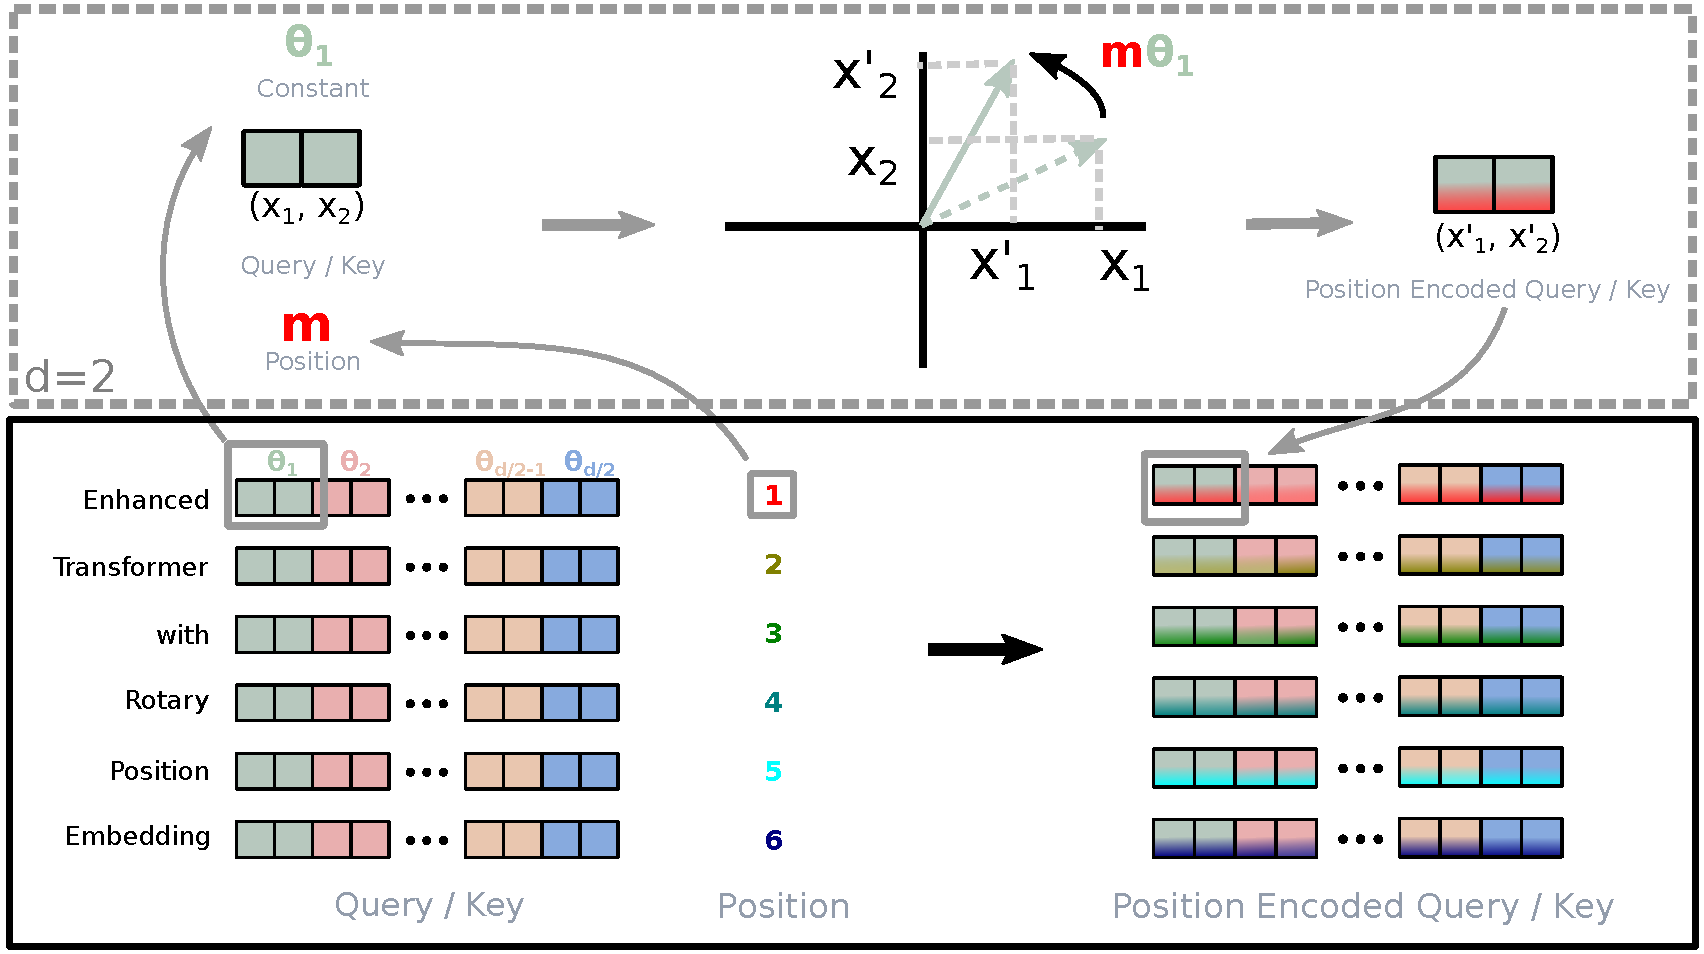
\includegraphics[width=0.84\linewidth,height=5.4cm,keepaspectratio]{fig-rope-paper}

\vspace{0.2em}
{\footnotesize\color{vnCite} Nguồn: \citet{Su2024}}
\end{frame}

% ---------------------------------------------------------------------
\begin{frame}{Pre-RMSNorm: gradient ổn định hơn, phép tính rẻ hơn}
\vspace{-0.35em}
\begin{columns}[T]
% ---------------- cột trái: vị trí đặt chuẩn hóa ----------------
\begin{column}{0.40\textwidth}
\centering
\resizebox{\ifdim\width>\linewidth\linewidth\else\width\fi}{!}{%
\begin{tikzpicture}[
  bx/.style={draw=vnNavy,fill=vnLight,rounded corners=2pt,text width=1.75cm,
             align=center,font=\scriptsize,minimum height=0.5cm,inner sep=2pt},
  nm/.style={bx,fill=white},
  pl/.style={draw=vnNavy,circle,inner sep=1.2pt,font=\scriptsize},
  ar/.style={-{Latex[length=1.4mm]},vnNavy,semithick}]

  % ---- Post-LN ----
  \node[font=\bfseries\scriptsize,text=vnNavy] at (0,4.55) {Post-LN (BERT)};
  \node[font=\scriptsize] (a0) at (0,0)     {$x$};
  \node[bx]               (a1) at (0,1.0)   {Lớp con};
  \node[pl]               (a2) at (0,2.0)   {$+$};
  \node[nm]               (a3) at (0,3.05)  {LayerNorm};
  \node[font=\scriptsize] (a4) at (0,3.95)  {$y$};
  \draw[ar] (a0)--(a1); \draw[ar] (a1)--(a2);
  \draw[ar] (a2)--(a3); \draw[ar] (a3)--(a4);
  \draw[ar] (a0.east) -- ++(1.3,0) |- (a2.east);
  \node[font=\tiny,text=vnCite,align=center] at (0,-0.75)
       {chuẩn hóa nằm \emph{trên}\\residual};

  % ---- Pre-RMSNorm ----
  \begin{scope}[xshift=3.9cm]
    \node[font=\bfseries\scriptsize,text=vnNavy] at (0,4.55) {Pre-RMSNorm};
    \node[font=\scriptsize] (b0) at (0,0)     {$x$};
    \node[nm]               (b1) at (0,1.0)   {RMSNorm};
    \node[bx]               (b2) at (0,2.05)  {Lớp con};
    \node[pl]               (b3) at (0,3.05)  {$+$};
    \node[font=\scriptsize] (b4) at (0,3.95)  {$y$};
    \draw[ar] (b0)--(b1); \draw[ar] (b1)--(b2);
    \draw[ar] (b2)--(b3); \draw[ar] (b3)--(b4);
    \draw[ar] (b0.east) -- ++(1.3,0) |- (b3.east);
    \node[font=\tiny,text=vnCite,align=center] at (0,-0.75)
         {residual \emph{thông suốt}\\từ đầu đến cuối};
  \end{scope}
\end{tikzpicture}}
\end{column}

% ---------------- cột phải: hai lý do ----------------
\begin{column}{0.575\textwidth}
\small
\lead{1. Đặt \emph{trước} $\Rightarrow$ gradient không phình ở lớp cuối}
Chuẩn gradient tại lớp cuối $\|\partial\mathcal{L}/\partial W^{L,2}\|_F$
khi khởi tạo ($L$ lớp, $d$ chiều):
\vspace{-0.35em}
\[\textstyle
  \underbrace{\mathcal{O}\big(d\sqrt{\ln d}\big)}_{\text{Post-LN}}
  \qquad\text{so với}\qquad
  \underbrace{\mathcal{O}\big(d\sqrt{\ln d\,/\,L}\big)}_{\text{Pre-LN}}
\]
\vspace{-0.85em}

Post-LN chuẩn hóa lại residual ở \emph{mọi} lớp: gradient
\textbf{không nhỏ đi} khi mạng sâu thêm, buộc phải dùng
\textit{warm-up} tốc độ học. Pre-LN chia thêm $\sqrt{L}$ nên \hl{28 lớp} của
NeoBERT huấn luyện ổn định \cit{Xiong2020}

\vspace{0.15em}
\lead{2. Bỏ trung bình $\Rightarrow$ mỗi lớp rẻ hơn}
\vspace{-0.45em}
\[\textstyle
  \underbrace{\tfrac{a_i-\mu}{\sigma}g_i+b_i}_{\text{LayerNorm}}
  \;\longrightarrow\;
  \underbrace{\tfrac{a_i}{\mathrm{RMS}(a)}g_i}_{\text{RMSNorm}},\;
  \mathrm{RMS}(a)=\sqrt{\tfrac{1}{n}\textstyle\sum_i a_i^2}
\]
\vspace{-0.5em}
\begin{flushright}\cit{Zhang2019}\end{flushright}
\end{column}
\end{columns}
\end{frame}

% ---------------------------------------------------------------------
\begin{frame}{Ba đặc điểm của NeoBERT định hình cách chuyển giao}
\vspace{0.4em}
\begin{columns}[T]
\begin{column}{0.48\textwidth}
  \lead{1. RoPE -- thuận lợi}
  \begin{itemize}\itemsep2pt
    \item Vị trí được áp \emph{bên trong} mỗi lớp, \textbf{không nằm} trong
          ma trận véc-tơ.
    \item[$\Rightarrow$] Thay toàn bộ lớp từ vựng tiếng Việt
          \emph{không đụng chạm} cơ chế vị trí.
  \end{itemize}
\end{column}

\begin{column}{0.48\textwidth}
  \lead{2. Pre-RMSNorm -- ràng buộc}
  \begin{itemize}\itemsep2pt
    \item Chuẩn hóa chia theo \emph{độ lớn} véc-tơ; lớp véc-tơ đi thẳng vào
          luồng chính qua residual.
    \item[$\Rightarrow$] Nếu độ lớn véc-tơ mới lệch khỏi thống kê NeoBERT,
          sai lệch bị khuếch đại qua 28 lớp.
  \end{itemize}
\end{column}
\end{columns}

\vspace{0.9em}
\begin{alertblock}{3. Lớp đầu ra không dùng chung trọng số}
  Khác BERT/RoBERTa, đầu MLM của NeoBERT là một ma trận \emph{độc lập} với
  ma trận véc-tơ đầu vào. Vì vậy chuyển sang tiếng Việt phải khởi tạo
  \hl{cả hai ma trận}, mỗi ma trận trong đúng không gian của nó.
\end{alertblock}
\end{frame}

% ---------------------------------------------------------------------
\begin{frame}{Đổi ngôn ngữ: khởi tạo lớp véc-tơ thế nào?}
\vspace{0.4em}
\centering
% Diagram is narrower than the text block, so \fitpic would leave it small.
% Force it up to 0.86\linewidth instead.
\resizebox{0.93\linewidth}{!}{\begin{tikzpicture}[font=\scriptsize,
  b/.style={draw=vnNavy,rounded corners=2pt,text width=2.6cm,
            minimum height=16mm,align=center,inner sep=3pt},
  ar/.style={-{Latex[length=2mm]},vnSteel,thick}]

  \node[b,fill=vnRed!10,draw=vnRed] (rnd)
       {\textbf{Ngẫu nhiên}\\[-1pt]\tiny tín hiệu vô nghĩa};
  \node[b,fill=vnLight,right=9mm of rnd] (sem)
       {\textbf{Theo ngữ nghĩa}\\[-1pt]\tiny WECHSEL, FOCUS, OFA};
  \node[b,fill=vnNavy,text=white,draw=vnNavy,right=9mm of sem] (salt)
       {\textbf{SALT}\\[-1pt]\tiny tái sử dụng không gian};

  \draw[ar] (rnd)--(sem);
  \draw[ar] (sem)--(salt);

  \node[below=3mm of rnd,text=vnRed,font=\tiny,align=center]
       {phá vỡ biểu diễn\\ đã có};
  \node[below=3mm of sem,text=vnCite,font=\tiny,align=center]
       {mượn \emph{véc-tơ tĩnh}\\ làm cầu nối};
  \node[below=3mm of salt,text=vnCite,font=\tiny,align=center]
       {mượn \emph{mô hình}\\ \emph{đã tiền huấn luyện}};
\end{tikzpicture}}

\vspace{1.0em}
\begin{columns}[T]
\begin{column}{0.94\textwidth}
  \small
  Khởi tạo ngẫu nhiên buộc phần thân học lại từ tín hiệu vô nghĩa
  \cit{deVries2021}. Các phương pháp theo ngữ nghĩa dùng véc-tơ tĩnh để bắc
  cầu; \textbf{SALT} đi xa hơn -- lấy thẳng không gian véc-tơ của một mô hình
  \hl{đã tiền huấn luyện} ở ngôn ngữ đích.
\end{column}
\end{columns}
\end{frame}

% ---------------------------------------------------------------------
\begin{frame}{SALT: tái sử dụng không gian véc-tơ của mô hình ngôn ngữ đích}
\vfill
\centering
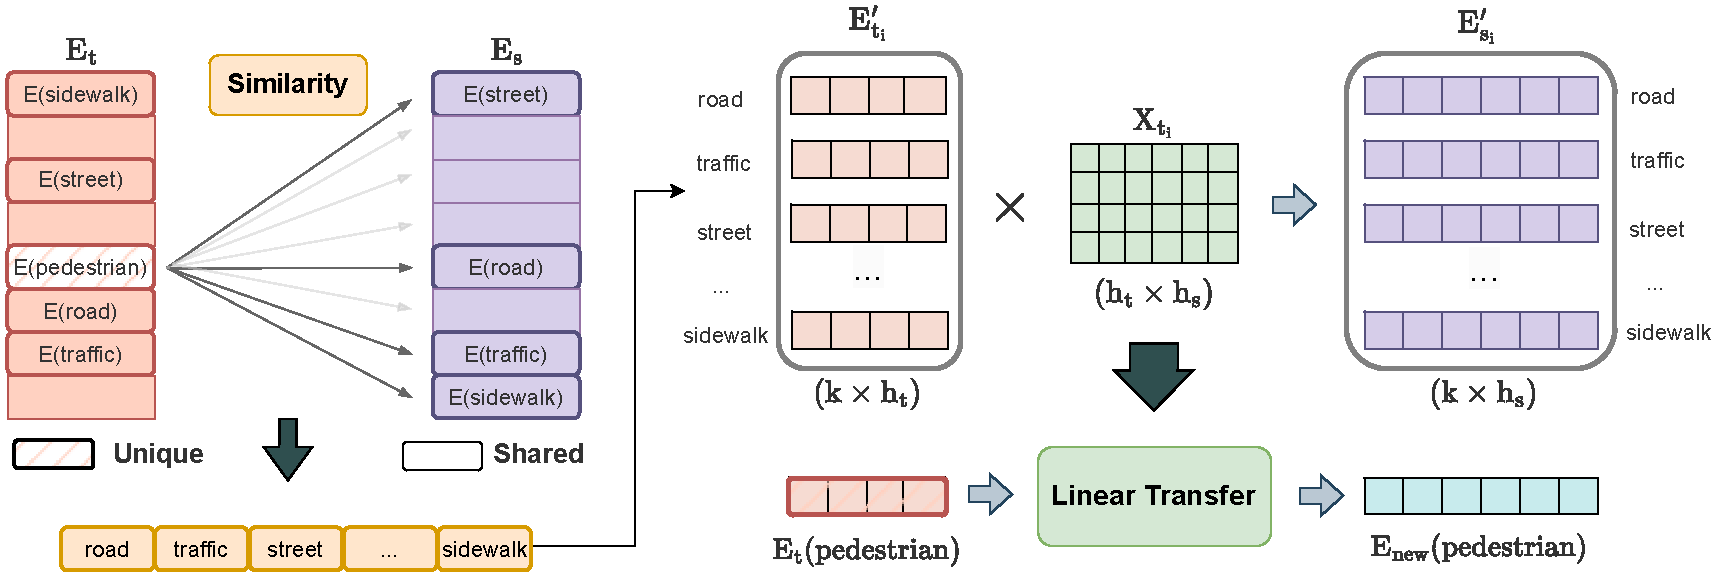
\includegraphics[width=\linewidth,height=5.9cm,keepaspectratio]{fig-salt-paper}

\vspace{0.4em}
{\footnotesize\color{vnCite} Nguồn: \citet{Lee2025}}
\vfill
\end{frame}

% =====================================================================
\section{Phương pháp đề xuất}
% =====================================================================
\subsection{Tổng quan}

% ---------------------------------------------------------------------
\begin{frame}{Quy trình xây dựng ViNeoBERT: ba giai đoạn}
\vspace{0.4em}
\centering
% Shrink only if the diagram would otherwise run past the text block.
\fitpic{\begin{tikzpicture}[font=\scriptsize,
  % text width (not just minimum width) so long labels wrap instead of
  % widening the node and colliding with its neighbour
  stage/.style={draw=vnNavy,fill=vnLight,rounded corners=2pt,
                text width=2.2cm,minimum height=11mm,align=center,inner sep=3pt},
  src/.style={draw=vnSteel,fill=white,rounded corners=2pt,
              text width=1.85cm,minimum height=8mm,align=center,inner sep=3pt}]

  \node[src] (neo) {NeoBERT\\[-1pt]\tiny kiến trúc + không gian đích};
  \node[src,below=7mm of neo] (vide) {ViDeBERTa\\[-1pt]\tiny mô hình nguồn véc-tơ};

  \node[stage,right=7mm of $(neo)!0.5!(vide)$] (s1)
       {\textbf{Giai đoạn 1}\\ Khởi tạo SALT\\[-1pt]\tiny thân đóng băng};
  \node[stage,right=4mm of s1] (s2)
       {\textbf{Giai đoạn 2}\\ Căn chỉnh\\[-1pt]\tiny thân đóng băng};
  \node[stage,right=4mm of s2] (s3)
       {\textbf{Giai đoạn 3}\\ CPT theo lịch WSD\\[-1pt]\tiny toàn bộ tham số};
  \node[src,right=5mm of s3,fill=vnNavy,text=white,draw=vnNavy] (out)
       {\textbf{ViNeoBERT}};

  \draw[-{Latex[length=2mm]},vnSteel,thick] (neo.east)  -- (s1.west|-neo)  -- (s1.west);
  \draw[-{Latex[length=2mm]},vnSteel,thick] (vide.east) -- (s1.west|-vide) -- (s1.west);
  \draw[-{Latex[length=2mm]},vnSteel,thick] (s1)--(s2);
  \draw[-{Latex[length=2mm]},vnSteel,thick] (s2)--(s3);
  \draw[-{Latex[length=2mm]},vnSteel,thick] (s3)--(out);

  \node[below=2mm of s1,text=vnCite,font=\tiny] {không huấn luyện};
  \node[below=2mm of s2,text=vnCite,font=\tiny] {$\sim$20 triệu token};
  \node[below=2mm of s3,text=vnCite,font=\tiny] {$\sim$5 tỷ token};
\end{tikzpicture}}

\vspace{0.8em}
\begin{columns}[T]
\begin{column}{0.95\textwidth}
\begin{alertblock}{Ba cải tiến của khóa luận so với SALT gốc}
  \small
  \begin{enumerate}\itemsep0pt
    \item \textbf{Mở rộng tập điểm neo} bằng các cặp dịch Anh--Việt khai thác tự động.
    \item \textbf{Khởi tạo riêng lớp đầu ra}, kèm hệ số điều chỉnh theo tần suất
          token và hệ số tỉ lệ $\gamma$.
    \item \textbf{Bổ sung giai đoạn căn chỉnh} với phần thân đóng băng trước khi
          huấn luyện toàn bộ.
  \end{enumerate}
\end{alertblock}
\end{column}
\end{columns}
\end{frame}

% ---------------------------------------------------------------------
\begin{frame}{Chọn ViDeBERTa làm mô hình nguồn véc-tơ}
\vspace{0.3em}
\begin{columns}[T]
\begin{column}{0.56\textwidth}
  \scriptsize
  \begin{tabular}{@{} L{2.3cm} L{2.2cm} L{2.7cm}@{}}
    \toprule
    \rowcolor{vnLight}
    \color{vnNavy}\bfseries Đặc điểm &
    \color{vnNavy}\bfseries PhoBERT &
    \color{vnNavy}\bfseries ViDeBERTa\\
    \midrule
    Token hóa      & BPE            & SentencePiece Unigram\\
    Từ vựng        & 64.000         & $\approx$128.000\\
    Đầu vào        & phải tách từ sẵn & \textbf{văn bản thô}\\
    Điểm log-xác suất & không có    & \textbf{có}\\
    Dữ liệu        & 20GB           & \textbf{$\approx$138GB}\\
    Điểm neo tiềm năng & hạn chế    & \textbf{phong phú}\\
    \bottomrule
  \end{tabular}
  \vspace{3pt}\\
  {\footnotesize\color{vnCite} So sánh theo \citet{Nguyen2020} và \citet{Tran2023}}

  \vspace{0.7em}
  {\footnotesize\color{vnCite} Lưu ý: SALT gốc dùng chính PhoBERT làm mô hình
   nguồn; khóa luận chủ đích đổi sang ViDeBERTa.}
\end{column}

\begin{column}{0.42\textwidth}
  \textbf{Ba lý do}
  \begin{itemize}\itemsep2pt
    \item Xử lý trực tiếp văn bản thô, không phụ thuộc công cụ tách từ
          bên ngoài.
    \item Từ vựng lớn hơn $\Rightarrow$ nhiều ứng viên điểm neo hơn.
    \item Học trên dữ liệu tiếng Việt lớn hơn nhiều $\Rightarrow$ không gian
          véc-tơ mã hóa ngữ nghĩa chính xác hơn.
  \end{itemize}

  \vspace{0.4em}
  \begin{block}{Giảm kích thước từ vựng}
    \small $128.000 \rightarrow \mathbf{30.522}$ token, giữ token đặc biệt và
    chọn theo điểm log-xác suất cao nhất -- để ViNeoBERT có số tham số ngang
    NeoBERT gốc.
  \end{block}
\end{column}
\end{columns}
\end{frame}

% ---------------------------------------------------------------------
\subsection{Tập điểm neo}

\begin{frame}{Tập điểm neo: cầu nối giữa hai không gian}
\vspace{0.3em}
\begin{columns}[T]
\begin{column}{0.44\textwidth}
  \lead{Điểm neo là gì?}

  Cặp token \emph{tương ứng ngữ nghĩa} giữa từ vựng tiếng Việt và tiếng Anh --
  mỗi cặp cho ta một điểm \emph{đã biết} của ánh xạ giữa hai không gian.

  \vspace{0.4em}
  \textbf{Hai vai trò}
  \begin{itemize}\itemsep1pt
    \item Token neo được khởi tạo bằng cách \emph{sao chép} véc-tơ NeoBERT.
    \item Các cặp neo làm \emph{tập giám sát} để học ánh xạ cho những token
          còn lại.
  \end{itemize}

  \vspace{0.3em}
  $\Rightarrow$ Số lượng và chất lượng điểm neo \hl{quyết định} chất lượng
  khởi tạo.
\end{column}

\begin{column}{0.53\textwidth}
  \small
  \begin{tabular}{@{} L{2.2cm} L{2.05cm} L{2.4cm}@{}}
    \toprule
    \rowcolor{vnLight}
    \color{vnNavy}\bfseries Nguồn &
    \color{vnNavy}\bfseries Ví dụ &
    \color{vnNavy}\bfseries Cách xác minh\\
    \midrule
    Trùng mặt chữ & \textit{internet} & dịch máy trả về chính nó\\[2pt]
    Chữ số        & \textit{2024}     & nhận trực tiếp\\[2pt]
    \rowcolor{vnLight}
    \textbf{Cặp dịch} & \textit{nước} $\leftrightarrow$ \textit{water}
                      & \textbf{đóng góp của khóa luận}\\
    \bottomrule
  \end{tabular}

  \vspace{0.6em}
  \begin{alertblock}{Bẫy: đồng tự khác nghĩa}
    \small Việt và Anh cùng dùng chữ Latin, nên trùng chuỗi \emph{chưa chắc}
    trùng nghĩa: \textit{song} (Việt: song song) $\neq$ \textit{song}
    (Anh: bài hát). Khóa luận lọc bằng dịch máy \cit{Junczys2018} --
    chỉ giữ khi bản dịch trùng chính chuỗi gốc.
  \end{alertblock}
\end{column}
\end{columns}
\end{frame}

% ---------------------------------------------------------------------
\begin{frame}{Mở rộng tập điểm neo bằng cặp dịch Anh--Việt}
\framesubtitle{Đóng góp chính ở bước khởi tạo}
\vspace{0.2em}
\begin{columns}[T]
\begin{column}{0.55\textwidth}
  \small
  Trước khi khai thác: lọc để chỉ giữ \textbf{từ tiếng Việt hợp lệ}
  (loại \textit{f, j, w, z}; đúng một cụm nguyên âm; tuân thủ quy tắc
  chính tả \textit{k/gh/ngh}, \textit{q}+\textit{u}\,\dots).

  \vspace{0.5em}
  \begin{tabular}{@{} L{1.0cm} L{3.3cm} L{2.85cm}@{}}
    \toprule
    \rowcolor{vnLight}
    \color{vnNavy}\bfseries Tầng &
    \color{vnNavy}\bfseries Cách khai thác &
    \color{vnNavy}\bfseries Ví dụ\\
    \midrule
    1 & Dịch ngược phải trùng từ gốc & sách $\to$ \textit{book} $\to$ sách\\[2pt]
    2 & Từ ghép, dịch một chiều      & bệnh viện $\to$ \textit{hospital}\\[2pt]
    3 & Từ đơn còn lại, lọc thủ công & bổ sung độ phủ\\
    \bottomrule
  \end{tabular}
\end{column}

\begin{column}{0.43\textwidth}
  \begin{block}{Vì sao dịch ngược lọc được từ đa nghĩa}
    \small Một từ đa nghĩa thường \emph{không} dịch ngược về chính nó, vì bản
    dịch trung gian ứng với một nghĩa khác. Ràng buộc dịch ngược trùng khớp
    do đó tự động giữ lại các cặp tương ứng một--một đáng tin cậy.
  \end{block}

  \vspace{0.3em}
  \textbf{Đánh đổi có chủ đích}
  \begin{itemize}\itemsep1pt
    \item Tầng 1 -- ưu tiên \emph{độ chính xác}.
    \item Tầng 2 -- tăng \emph{số lượng}; từ ghép ít đa nghĩa hơn từ đơn.
    \item Tầng 3 -- vét nốt \emph{độ phủ}.
  \end{itemize}
\end{column}
\end{columns}
\end{frame}

% ---------------------------------------------------------------------
\subsection{Khởi tạo SALT}

\begin{frame}{Khởi tạo mỗi token bằng một ánh xạ tuyến tính cục bộ}
\vspace{0.3em}
\begin{columns}[T]
\begin{column}{0.52\textwidth}
  \lead{Bước 1 -- chọn điểm neo gần nghĩa nhất}

  Đo tương đồng trong không gian véc-tơ tĩnh fastText \cit{Bojanowski2017},
  rồi lọc bằng \emph{sparsemax} \cit{Martins2016}:
  \vspace{-4pt}
  \[ s_{t,a}=\frac{f_t^{\top}f_a}{\|f_t\|\|f_a\|},\qquad
     w_t=\mathrm{sparsemax}(s_t) \]
  \vspace{-8pt}

  {\footnotesize Khác softmax, sparsemax đặt hẳn trọng số của các điểm neo
  xa nghĩa \emph{về 0} -- chỉ những điểm thực sự gần mới tham gia.}

  \vspace{0.5em}
  \textbf{Bước 2 -- học ánh xạ riêng cho token đó}
  \vspace{-4pt}
  \[ X_t=\bigl(A^{\mathrm{src}}_t\bigr)^{+}A^{\mathrm{tgt}}_t,
     \qquad e_t=d_t X_t \]
  \vspace{-8pt}

  {\footnotesize $X_t$ là ánh xạ khớp bình phương tối thiểu, đưa véc-tơ nguồn
  của các điểm neo về sát véc-tơ đích tương ứng.}
\end{column}

\begin{column}{0.45\textwidth}
  \begin{block}{Vì sao \emph{cục bộ} chứ không phải một ánh xạ chung}
    \small Hai không gian được huấn luyện độc lập nên \emph{không đẳng cấu}
    \cit{Ormazabal2019} và có tính bất đẳng hướng \cit{Ethayarajh2019}.
    Một ánh xạ tuyến tính duy nhất cho cả từ vựng là không đủ; mỗi token
    được chiếu dựa trên chính các điểm neo lân cận nó.
  \end{block}

  \vspace{0.4em}
  \textbf{Các trường hợp còn lại}
  \begin{itemize}\itemsep1pt
    \item Ít hơn $k_0=8$ điểm neo $\Rightarrow$ dùng trung bình có trọng số
          của các véc-tơ đích.
    \item Không có véc-tơ fastText $\Rightarrow$ lấy mẫu ngẫu nhiên khớp
          thống kê NeoBERT.
  \end{itemize}
\end{column}
\end{columns}
\end{frame}

% ---------------------------------------------------------------------
\begin{frame}{Chiếu riêng cho cả hai ma trận -- khác biệt so với SALT gốc}
\vspace{0.3em}
\begin{columns}[T]
\begin{column}{0.50\textwidth}
  Vì lớp đầu ra của NeoBERT \emph{không} dùng chung trọng số với lớp véc-tơ
  đầu vào, hai ma trận có \textbf{hình học riêng} và phải được khởi tạo
  độc lập:

  \vspace{0.4em}
  \begin{itemize}\itemsep2pt
    \item \textbf{Ma trận véc-tơ $E$}: véc-tơ đích lấy từ các véc-tơ
          \emph{đầu vào} NeoBERT của điểm neo.
    \item \textbf{Ma trận đầu ra $W_{\mathrm{dec}}$}: véc-tơ đích lấy từ các
          véc-tơ \emph{đầu ra} NeoBERT của cùng tập điểm neo.
  \end{itemize}

  \vspace{0.5em}
  {\footnotesize Sao chép ma trận véc-tơ sang lớp đầu ra -- thói quen kế thừa
  từ các kiến trúc dùng chung trọng số -- gây hại vì hai lớp đảm nhận hai vai
  trò hình học khác nhau \cit{Gao2019}. Thực nghiệm ở phần sau xác nhận
  điều này.}
\end{column}

\begin{column}{0.47\textwidth}
\centering
\fitpic{\begin{tikzpicture}[font=\scriptsize,
  m/.style={draw=vnNavy,rounded corners=2pt,minimum width=2.4cm,
            minimum height=8mm,align=center}]
  \node[m,fill=vnSteel!12] (anchor) {Tập điểm neo\\[-1pt]\tiny dùng chung};
  \node[m,fill=vnLight,below left=9mm and -6mm of anchor] (e) {SALT $\to E$};
  \node[m,fill=vnLight,below right=9mm and -6mm of anchor] (w)
       {SALT $\to W_{\mathrm{dec}}$};
  \node[below=5mm of e,text=vnCite,font=\tiny,align=center]
       {không gian\\véc-tơ đầu vào};
  \node[below=5mm of w,text=vnCite,font=\tiny,align=center]
       {không gian\\véc-tơ đầu ra};
  \draw[-{Latex[length=2mm]},vnSteel,thick] (anchor)--(e);
  \draw[-{Latex[length=2mm]},vnSteel,thick] (anchor)--(w);
\end{tikzpicture}}

\vspace{0.5em}
\begin{alertblock}{Kết quả sớm}
  \small Khởi tạo riêng hai ma trận đạt \hl{67,52} điểm F1, so với
  \textbf{54,09} khi dùng chung trọng số.
\end{alertblock}
\end{column}
\end{columns}
\end{frame}

% ---------------------------------------------------------------------
\begin{frame}{Ba bước tinh chỉnh sau khi chiếu}
\vspace{0.4em}
\begin{columns}[T]
\begin{column}{0.315\textwidth}
  \begin{block}{1. Hiệu chỉnh độ lớn}
    \small
    \[ e_t \leftarrow e_t\cdot\frac{\mu_{\mathrm{neo}}}{\|e_t\|} \]
    Đưa mỗi véc-tơ về \emph{độ lớn trung bình} của NeoBERT, giữ nguyên hướng.

    \vspace{2pt}
    {\footnotesize Cần thiết vì Pre-RMSNorm nhạy với độ lớn đầu vào.}
  \end{block}
\end{column}

\begin{column}{0.335\textwidth}
  \begin{block}{2. Bias theo tần suất token}
    \small
    \[ b_{\mathrm{dec},v}=\log p_v \]
    Khởi tạo bias đầu ra bằng log-tần-suất token tiếng Việt
    \cit{Meister2023}.

    \vspace{2pt}
    {\footnotesize Mô hình khỏi tốn hàng nghìn bước chỉ để học lại phân phối
    tần suất.}
  \end{block}
\end{column}

\begin{column}{0.315\textwidth}
  \begin{block}{3. Thu nhỏ trọng số đầu ra}
    \small
    \[ y=\gamma\,W_{\mathrm{dec}}h+b_{\mathrm{dec}},\;\; \gamma=0{,}1 \]
    Để tín hiệu tần suất \emph{chi phối} giai đoạn đầu.

    \vspace{2pt}
    {\footnotesize Nhân vô hướng nên vẫn giữ nguyên hướng ngữ nghĩa mà SALT
    dựng được.}
  \end{block}
\end{column}
\end{columns}

\vspace{0.5em}
\begin{block}{Kết quả của ba bước: điểm xuất phát tốt hơn hẳn}
  \small
  Mất mát khởi điểm xấp xỉ \textbf{entropy unigram tiếng Việt}
  ($\approx$7,3 nat) thay vì mức đoán ngẫu nhiên $\log|V_t|\approx$
  \textbf{10,3 nat} -- tức mô hình bắt đầu từ chỗ \emph{đã biết} phân phối
  từ vựng tiếng Việt.
\end{block}
\end{frame}

% ---------------------------------------------------------------------
\subsection{Huấn luyện}

\begin{frame}{Giai đoạn 2 và 3: căn chỉnh rồi mới huấn luyện toàn bộ}
\vspace{0.3em}
\begin{columns}[T]
\begin{column}{0.47\textwidth}
  \textbf{Giai đoạn 2 -- căn chỉnh với thân đóng băng}
  \begin{itemize}\itemsep1pt
    \item Đóng băng toàn bộ 28 lớp; chỉ huấn luyện hai ma trận mới trên
          $\sim$20 triệu token.
    \item Để hai ma trận \emph{khớp với nhau và với phần thân} trước khi cho
          phần thân thay đổi \cit{deVries2021}.
    \item Chi phí không đáng kể, nhưng giảm $\approx$26\% perplexity.
  \end{itemize}

  \vspace{0.5em}
  \textbf{Giai đoạn 3 -- tiếp tục tiền huấn luyện}
  \begin{itemize}\itemsep1pt
    \item Toàn bộ tham số, $\sim$5 tỷ token CulturaX tiếng Việt
          \cit{Nguyen2024}.
    \item Khởi động lại tốc độ học khi huấn luyện tiếp \cit{Ibrahim2024}.
  \end{itemize}
\end{column}

\begin{column}{0.49\textwidth}
\centering
\fitpic{\begin{tikzpicture}[font=\scriptsize,x=1cm,y=1cm]
  \draw[->,vnCite] (0,0)--(6.15,0) node[below left=1pt and -2pt,font=\tiny]{bước $s$};
  \draw[->,vnCite] (0,0)--(0,2.1) node[above,font=\tiny]{$\eta$};
  \draw[vnNavy,very thick] (0,0)--(0.9,1.6);
  \draw[vnNavy,very thick] (0.9,1.6)--(4.3,1.6);
  \draw[vnNavy,very thick] (4.3,1.6)
        .. controls (5.1,1.45) and (5.4,0.7) .. (5.9,0);
  \draw[vnSteel,thick,dashed] (2.9,1.6)
        .. controls (3.5,1.35) and (3.7,0.6) .. (4.1,0);
  \node[text=vnNavy,font=\tiny] at (0.45,1.85) {khởi động};
  \node[text=vnNavy,font=\tiny] at (2.6,1.82) {ổn định};
  \node[text=vnNavy,font=\tiny] at (5.7,1.15) {làm nguội};
  \node[text=vnSteel,font=\tiny,align=center] at (3.35,0.42)
       {nhánh\\giữa chừng};
\end{tikzpicture}}

\vspace{2pt}
{\footnotesize\color{vnCite} Lịch tốc độ học Warmup--Stable--Decay
 \citep{Hu2024}}

\vspace{0.3em}
\begin{block}{Vì sao chọn WSD thay vì cosine}
  \small Lịch cosine buộc phải \emph{cam kết trước} tổng số bước. WSD cho phép
  rẽ một nhánh làm nguội ngắn tại bất kỳ mốc nào để lấy mô hình hoàn chỉnh,
  trong khi nhánh chính vẫn tiếp tục -- rất hợp với việc đo chất lượng theo
  từng mốc ngân sách.
\end{block}
\end{column}
\end{columns}
\end{frame}

% =====================================================================
\section{Thực nghiệm và đánh giá}
% =====================================================================
\subsection{Thiết lập}

% ---------------------------------------------------------------------
\begin{frame}{Thiết lập thực nghiệm}
\vspace{0.3em}
\begin{columns}[T]
\begin{column}{0.40\textwidth}
  \textbf{Môi trường}
  \begin{itemize}\itemsep1pt
    \item GPU NVIDIA A100 80GB (Google Colab).
    \item PyTorch + hệ sinh thái Hugging Face.
  \end{itemize}

  \vspace{0.5em}
  \textbf{Dữ liệu}
  \begin{itemize}\itemsep1pt
    \item Căn chỉnh: $\sim$20 triệu token CulturaX-vi.
    \item CPT: $\sim$5 tỷ token ($\sim$20GB văn bản), đi qua \emph{đúng một lượt}.
    \item Mở rộng ngữ cảnh: $\sim$200 triệu token ở độ dài 4.096.
  \end{itemize}

  \vspace{0.4em}
  {\footnotesize\color{vnCite} Mọi kết quả tinh chỉnh lấy trung bình 5 seed
   ngẫu nhiên, báo cáo kèm độ lệch chuẩn.}
\end{column}

\begin{column}{0.58\textwidth}
  \scriptsize
  \begin{tabular}{@{}l r l r r@{}}
    \toprule
    \rowcolor{vnLight}
    \color{vnNavy}\bfseries Mô hình & \color{vnNavy}\bfseries Tham số &
    \color{vnNavy}\bfseries Kiến trúc & \color{vnNavy}\bfseries Token vi &
    \color{vnNavy}\bfseries Ngữ cảnh\\
    \midrule
    PhoBERT-base      & 135M & RoBERTa & $\sim$140 tỷ & 512\\
    PhoBERT-base-v2   & 135M & RoBERTa & $>$140 tỷ    & 512\\
    PhoBERT-large     & 370M & RoBERTa & $\sim$140 tỷ & 512\\
    XLM-R-base        & 278M & RoBERTa & hàng trăm tỷ & 512\\
    XLM-R-large       & 560M & RoBERTa & hàng trăm tỷ & 512\\
    \ourrow
    \textbf{ViNeoBERT} & \textbf{$\approx$250M} & \textbf{NeoBERT} &
    \hl{5 tỷ} & \textbf{4.096}\\
    \bottomrule
  \end{tabular}

  \vspace{4pt}
  {\footnotesize\color{vnCite} Các mô hình so sánh
   \citep{Nguyen2020,Conneau2020}}

  \vspace{0.5em}
  \begin{block}{Điểm cần chú ý khi đọc mọi kết quả sau}
    \small ViNeoBERT chỉ tiếp xúc \hl{3,5\%} lượng token tiếng Việt mà
    PhoBERT-large đã huấn luyện.
  \end{block}
\end{column}
\end{columns}
\end{frame}

% ---------------------------------------------------------------------
\begin{frame}{Bộ đánh giá: 12 tác vụ trên 5 nhóm năng lực}
\vspace{0.3em}
\begin{columns}[T]
\begin{column}{0.56\textwidth}
  \scriptsize
  \begin{tabular}{@{} L{2.5cm} L{2.9cm} L{1.9cm}@{}}
    \toprule
    \rowcolor{vnLight}
    \color{vnNavy}\bfseries Nhóm năng lực &
    \color{vnNavy}\bfseries Bộ dữ liệu &
    \color{vnNavy}\bfseries Độ đo\\
    \midrule
    Hỏi đáp đọc hiểu    & UIT-ViQuAD 2.0            & EM, F1\\
    Suy luận            & XNLI, ViANLI, QNLI        & Acc, F1-macro\\
    Phân loại văn bản   & UIT-VSFC, VSMEC, ViCTSD   & F1\\
    Chấp nhận ngữ pháp  & ViCoLA-syn                & MCC\\
    Gán nhãn từ loại    & UD-VTB                    & F1-macro\\
    Tương đồng ngữ nghĩa& STS, Paraphrase           & Spearman, F1\\
    Biểu diễn câu       & Retrieval, Reranking      & nDCG@10, MRR\\
    \bottomrule
  \end{tabular}
\end{column}

\begin{column}{0.42\textwidth}
  \textbf{Hai câu hỏi nghiên cứu}

  \vspace{0.3em}
  \begin{block}{Câu hỏi 1}
    \small Phương án \emph{khởi tạo} nào tốt nhất?\\
    $\rightarrow$ so sánh có kiểm soát, cùng ngân sách token.
  \end{block}

  \begin{block}{Câu hỏi 2}
    \small Mô hình cuối đạt chất lượng ra sao so với các mô hình hiện có?\\
    $\rightarrow$ đường cong theo ngân sách + bảng 12 tác vụ.
  \end{block}

  \vspace{0.2em}
  {\footnotesize\color{vnCite} UIT-ViQuAD được chọn làm thước đo quyết định vì
   nó buộc mô hình dùng đến ngữ nghĩa thực sự của từng token.}
\end{column}
\end{columns}
\end{frame}

% ---------------------------------------------------------------------
\subsection{So sánh khởi tạo}

\begin{frame}{SALT có thực sự đưa từ vựng tiếng Việt vào đúng không gian?}
\vspace{0.2em}
\begin{columns}[T]
\begin{column}{0.60\textwidth}
  \centering
  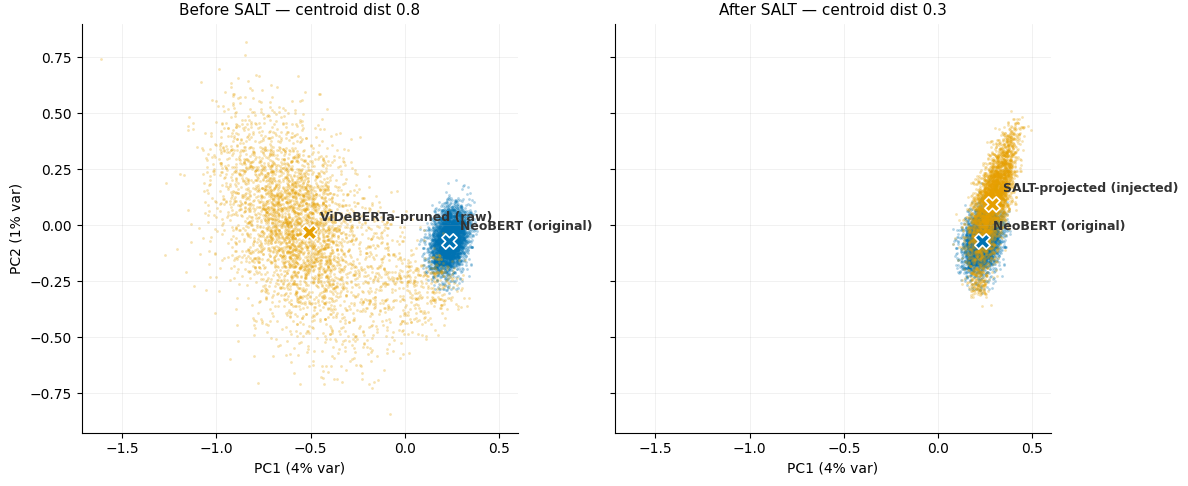
\includegraphics[width=\linewidth]{fig-pca-salt}\\[2pt]
  {\footnotesize\color{vnCite} Hình: lớp véc-tơ tiếng Việt trước và sau SALT,
   chiếu bằng PCA trên \emph{cùng một hệ trục}}
\end{column}

\begin{column}{0.38\textwidth}
  \textbf{Cách đọc hình}
  \begin{itemize}\itemsep1pt
    \item Vàng: véc-tơ tiếng Việt (ViDeBERTa). Xanh: véc-tơ NeoBERT gốc.
    \item Token điểm neo \emph{đã bị loại khỏi hình} -- chúng vốn được sao
          chép nguyên vẹn nên sẽ tạo vùng chồng lấp giả tạo.
  \end{itemize}

  \vspace{0.4em}
  \textbf{Kết quả}
  \begin{itemize}\itemsep1pt
    \item Khoảng cách hai tâm giảm từ \textbf{0,8} còn \hl{0,3}; độ trải cũng
          thu về khớp với NeoBERT.
    \item[$\Rightarrow$] Phép chiếu đưa từ vựng tiếng Việt về đúng vùng mà
          phần thân được huấn luyện để xử lý.
  \end{itemize}
\end{column}
\end{columns}
\end{frame}

% ---------------------------------------------------------------------
\begin{frame}{Hệ số tỉ lệ trọng số đầu ra $\gamma$ là bắt buộc}
\vspace{0.2em}
\begin{columns}[T]
\begin{column}{0.55\textwidth}
  \centering
  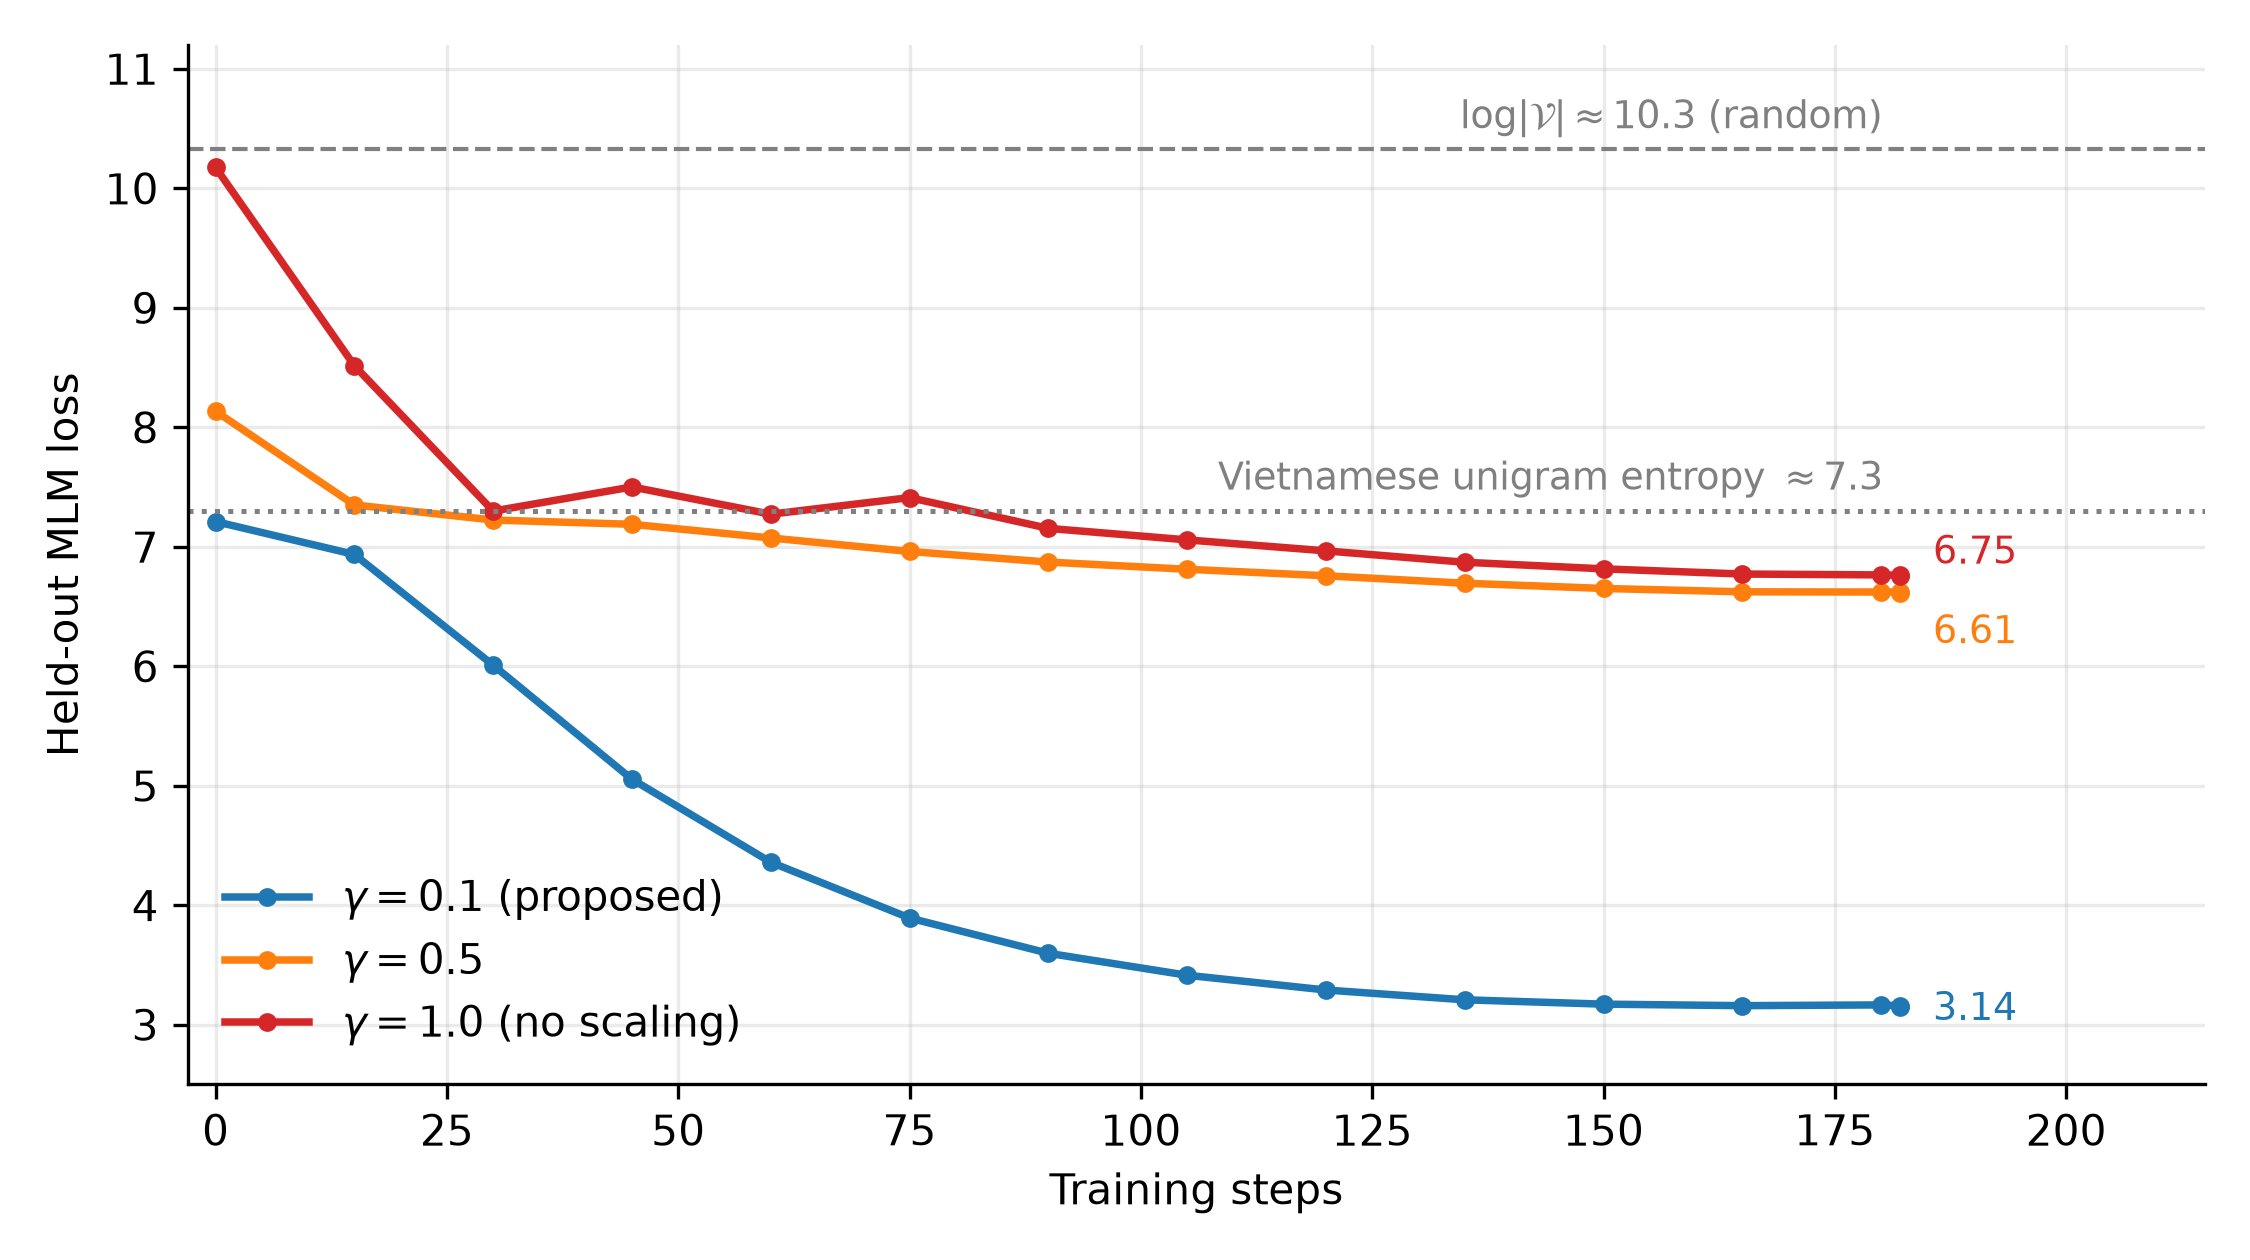
\includegraphics[width=\linewidth]{fig-gamma-loss}\\[2pt]
  {\footnotesize\color{vnCite} Hình: mất mát MLM theo hệ số tỉ lệ $\gamma$}
\end{column}

\begin{column}{0.43\textwidth}
  \small
  Ba phương án \emph{giống hệt nhau} về khởi tạo, chỉ khác đúng $\gamma$.

  \vspace{0.4em}
  \begin{tabular}{@{}l r r@{}}
    \toprule
    \rowcolor{vnLight}
    \color{vnNavy}\bfseries $\gamma$ &
    \color{vnNavy}\bfseries Mất mát đầu &
    \color{vnNavy}\bfseries Chuẩn grad\\
    \midrule
    1{,}0 & 10,18 & 68,4\\
    0{,}5 & 8,13  & 15,8\\
    \ourrow \textbf{0{,}1} & \textbf{7,21} & \textbf{2,1}\\
    \bottomrule
  \end{tabular}

  \vspace{0.5em}
  \begin{itemize}\itemsep1pt
    \item $\gamma$ lớn: logit \emph{nhiễu} từ ma trận vừa chiếu lấn át tín
          hiệu tần suất; cập nhật đầu tiên biên độ rất lớn nhưng ít thông
          tin $\Rightarrow$ \textbf{mắc kẹt} quanh 6,6--6,8.
    \item $\gamma=0{,}1$: khởi đầu ngay tại entropy unigram rồi hội tụ về
          \hl{3,14}.
  \end{itemize}
\end{column}
\end{columns}
\end{frame}

% ---------------------------------------------------------------------
\begin{frame}{So sánh năm phương án khởi tạo ở cùng ngân sách}
\vspace{0.1em}
\centering
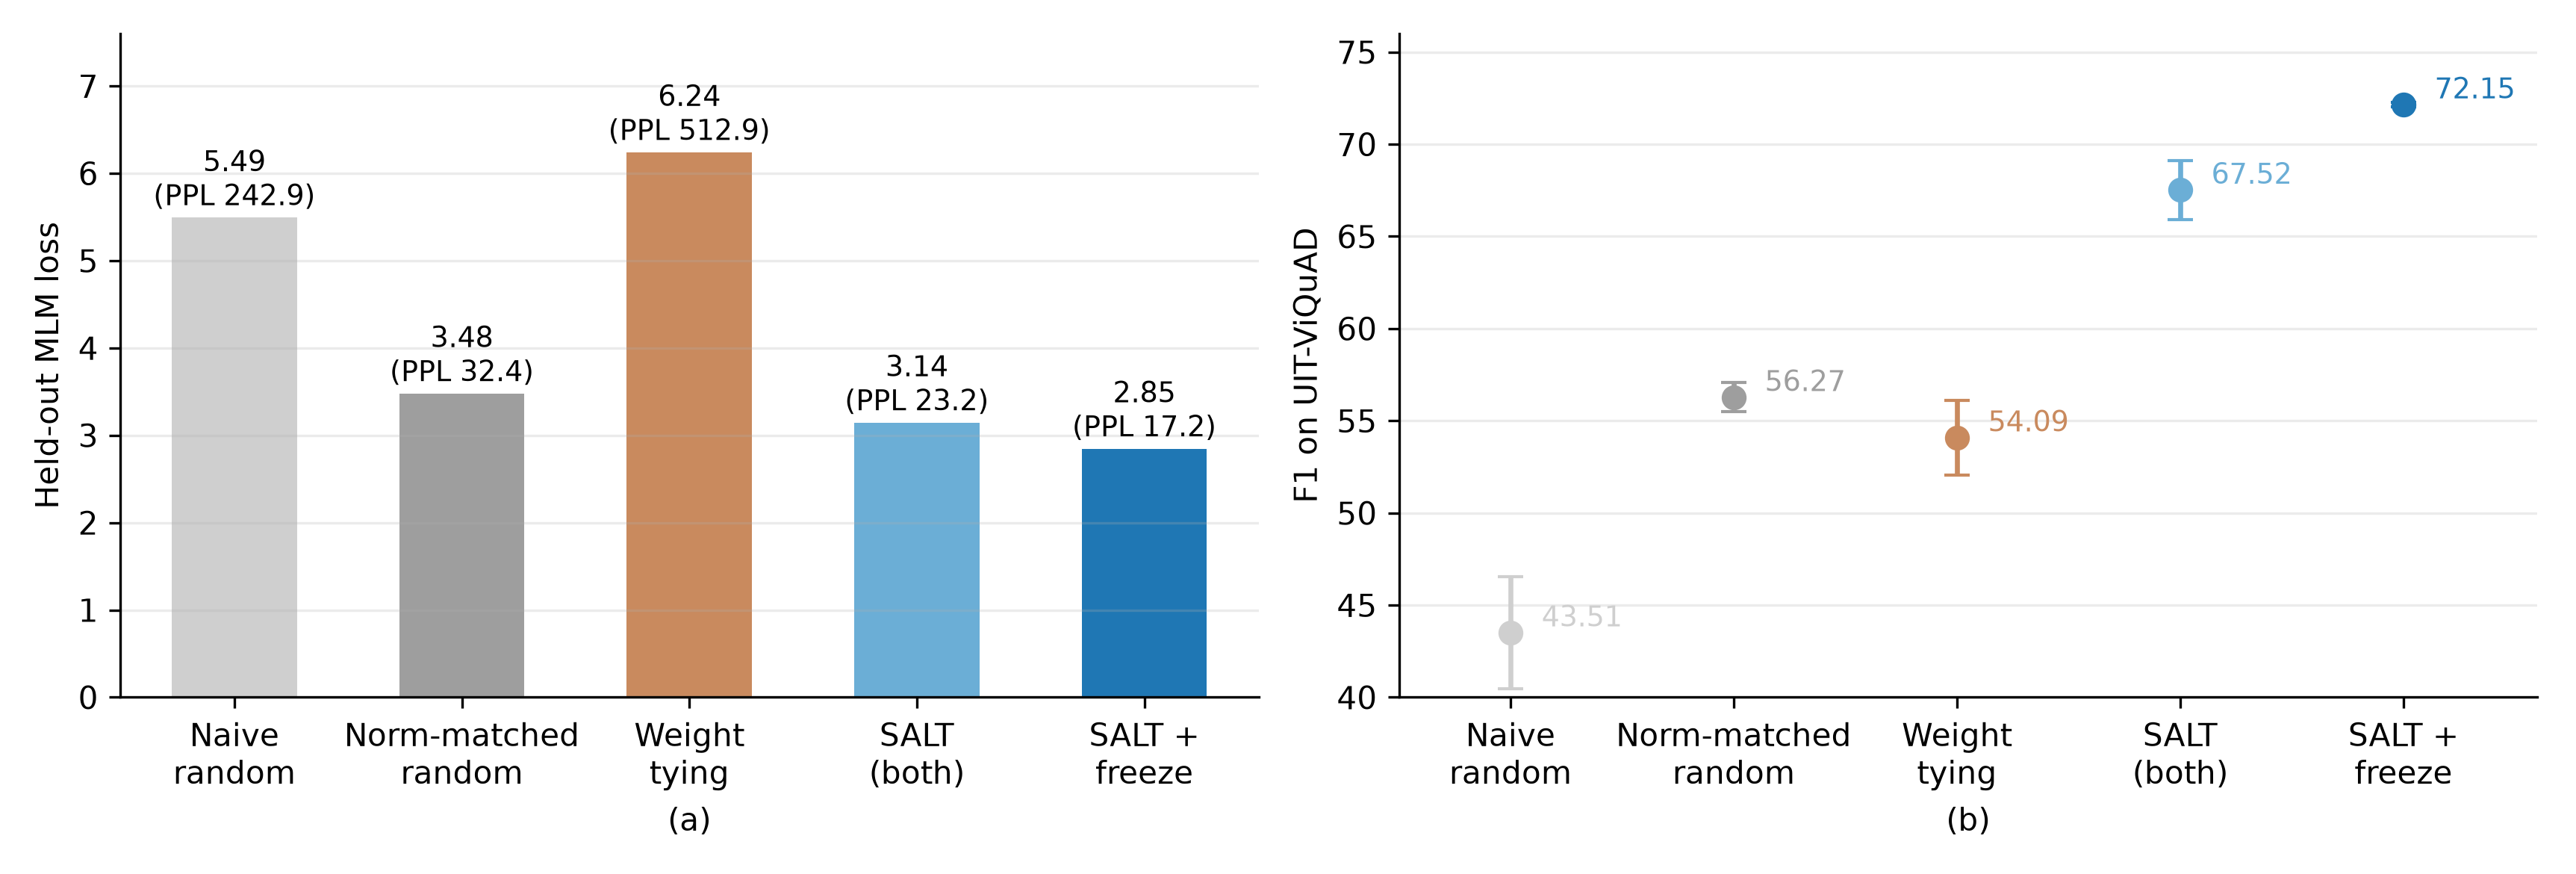
\includegraphics[width=0.78\linewidth]{fig-init-compare}\\[1pt]
{\footnotesize\color{vnCite} (a) mất mát MLM trên tập đánh giá\quad
 (b) F1 trên UIT-ViQuAD tại mốc 100 triệu token, thanh lỗi qua 3 seed}

\vspace{0.3em}
\begin{columns}[T]
\begin{column}{0.48\textwidth}
  \begin{alertblock}{Giá trị của hướng ngữ nghĩa}
    \footnotesize Đường cơ sở \emph{khớp mô-men} đã có đúng độ lớn, ánh xạ đầu
    ra và hệ số tần suất -- chỉ thiếu \emph{hướng} véc-tơ. Khoảng cách
    \hl{$+11{,}2$ điểm} vì thế quy hết về phần lõi của phương pháp.
  \end{alertblock}
\end{column}

\begin{column}{0.48\textwidth}
  \begin{block}{Dùng chung trọng số gây hại}
    \footnotesize 54,09 so với 56,27 -- hai lớp có vai trò hình học khác nhau.
    Căn chỉnh với thân đóng băng nâng tiếp lên \textbf{72,15}, độ lệch chuẩn
    giảm hơn một bậc (1,61 $\to$ 0,12).
  \end{block}
\end{column}
\end{columns}
\end{frame}

% ---------------------------------------------------------------------
\subsection{Kết quả mô hình}

\begin{frame}{Quá trình huấn luyện: khởi đầu thấp, hội tụ nhanh}
\vspace{0.2em}
\begin{columns}[T]
\begin{column}{0.58\textwidth}
  \centering
  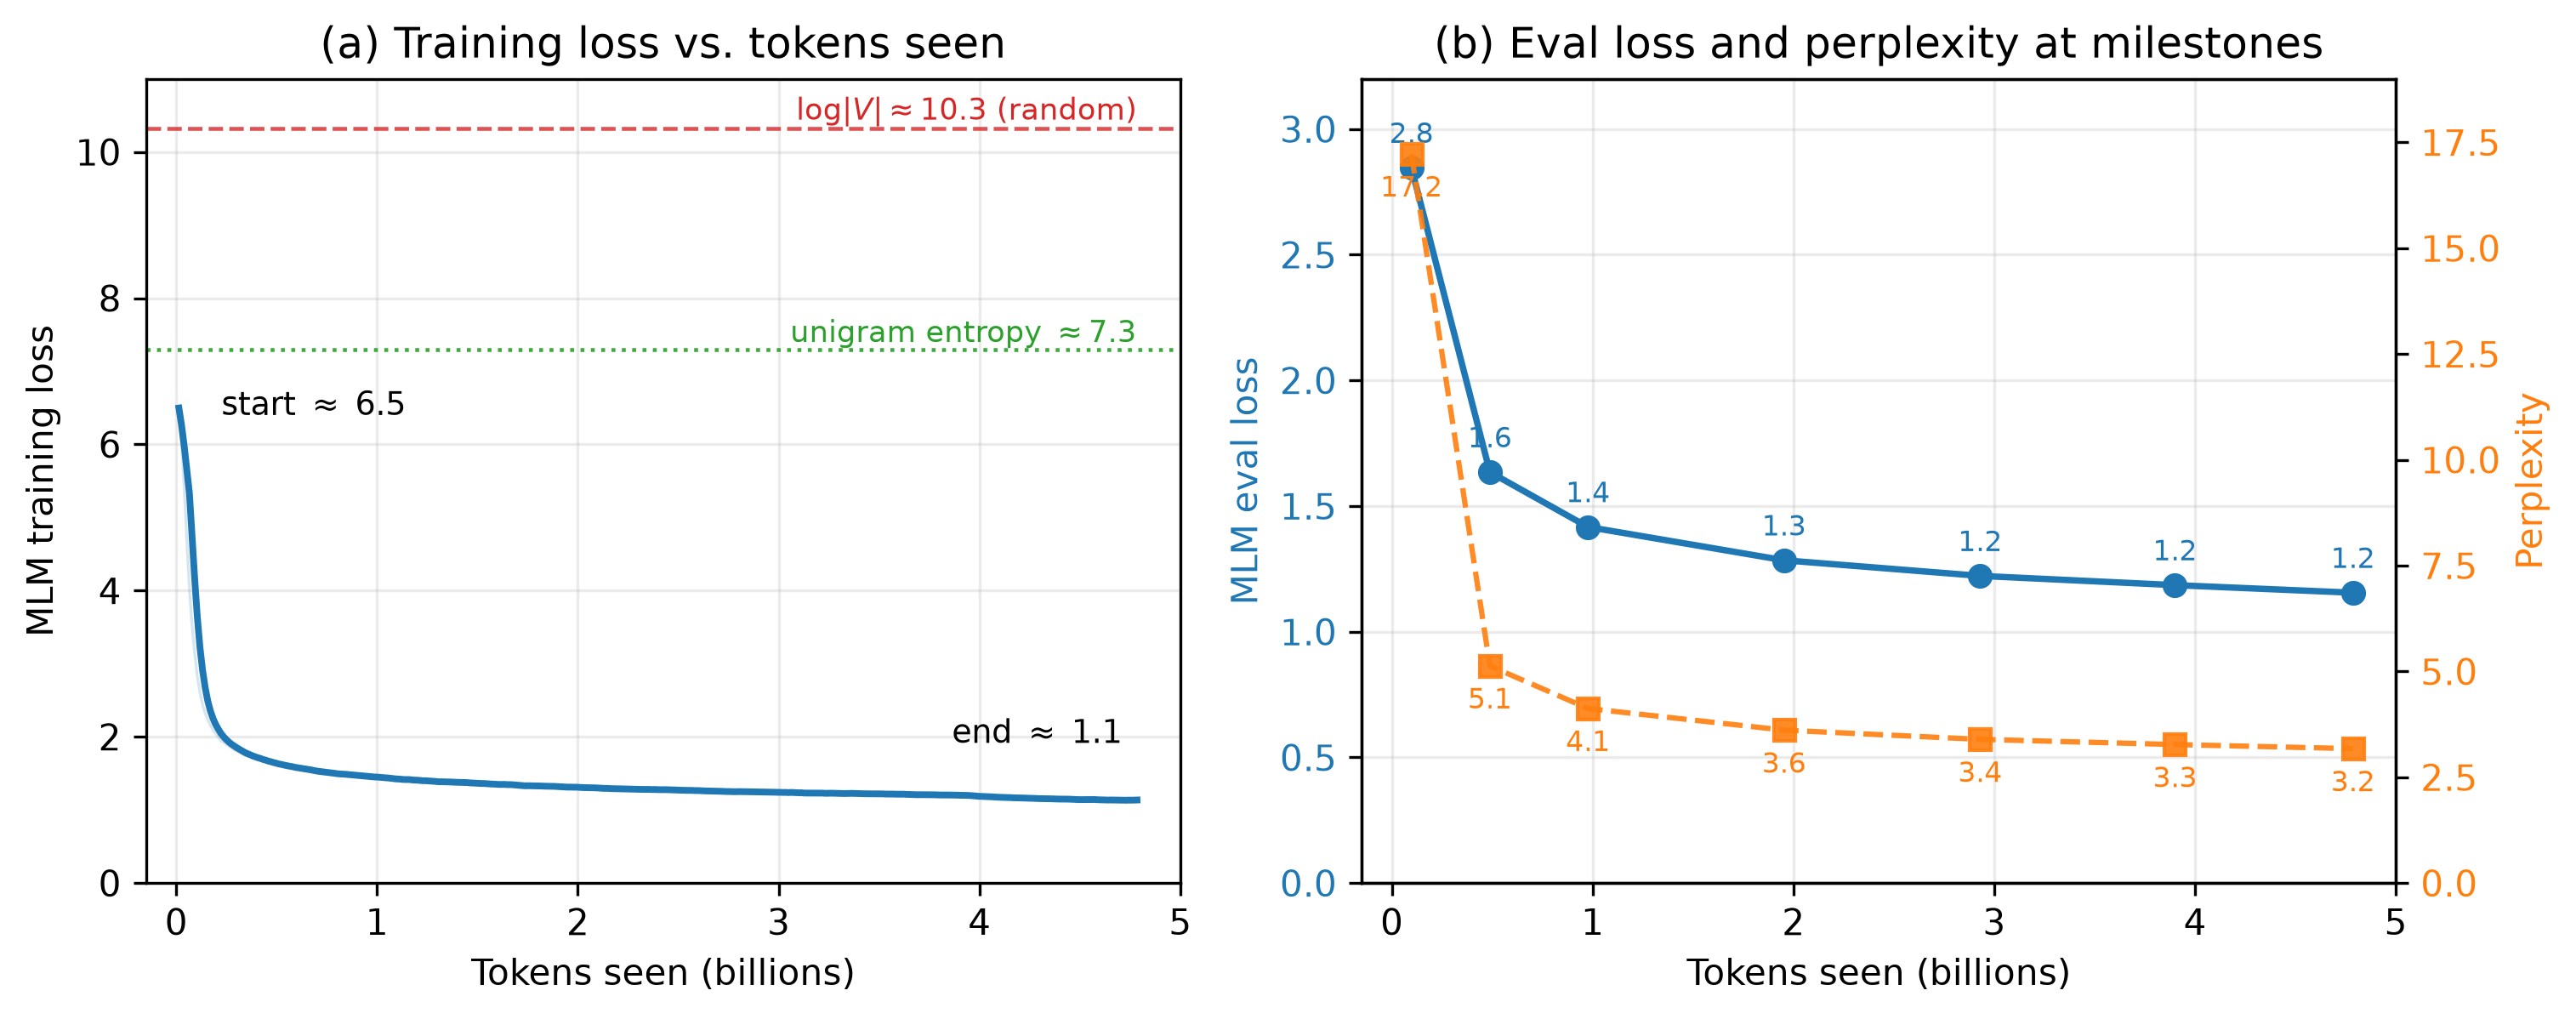
\includegraphics[width=\linewidth]{fig-cpt-loss}\\[2pt]
  {\footnotesize\color{vnCite} Hình: đường cong mất mát giai đoạn CPT
   theo lịch WSD}
\end{column}

\begin{column}{0.40\textwidth}
  \begin{itemize}\itemsep2pt
    \item Nhờ khởi tạo SALT, mất mát bắt đầu ở $\approx$\textbf{6,5} -- đã
          nằm \emph{dưới} mức đoán ngẫu nhiên ($\approx$10,3) và gần entropy
          unigram tiếng Việt ($\approx$7,3).
    \item Chỉ trong \textbf{0,2 tỷ token} đầu, mất mát đã rơi xuống dưới 2,0.
    \item Pha làm nguội cuối kéo mất mát về $\approx$\textbf{1,1};
          perplexity trên tập đánh giá giảm còn \hl{3,2}.
  \end{itemize}

  \vspace{0.4em}
  {\footnotesize $\Rightarrow$ Phần thân kế thừa từ NeoBERT \emph{không phải}
   học lại tiếng Việt từ đầu.}
\end{column}
\end{columns}
\end{frame}

% ---------------------------------------------------------------------
\begin{frame}{Phần lớn chất lượng đến từ những trăm triệu token đầu tiên}
\vspace{0.2em}
\begin{columns}[T]
\begin{column}{0.55\textwidth}
  \centering
  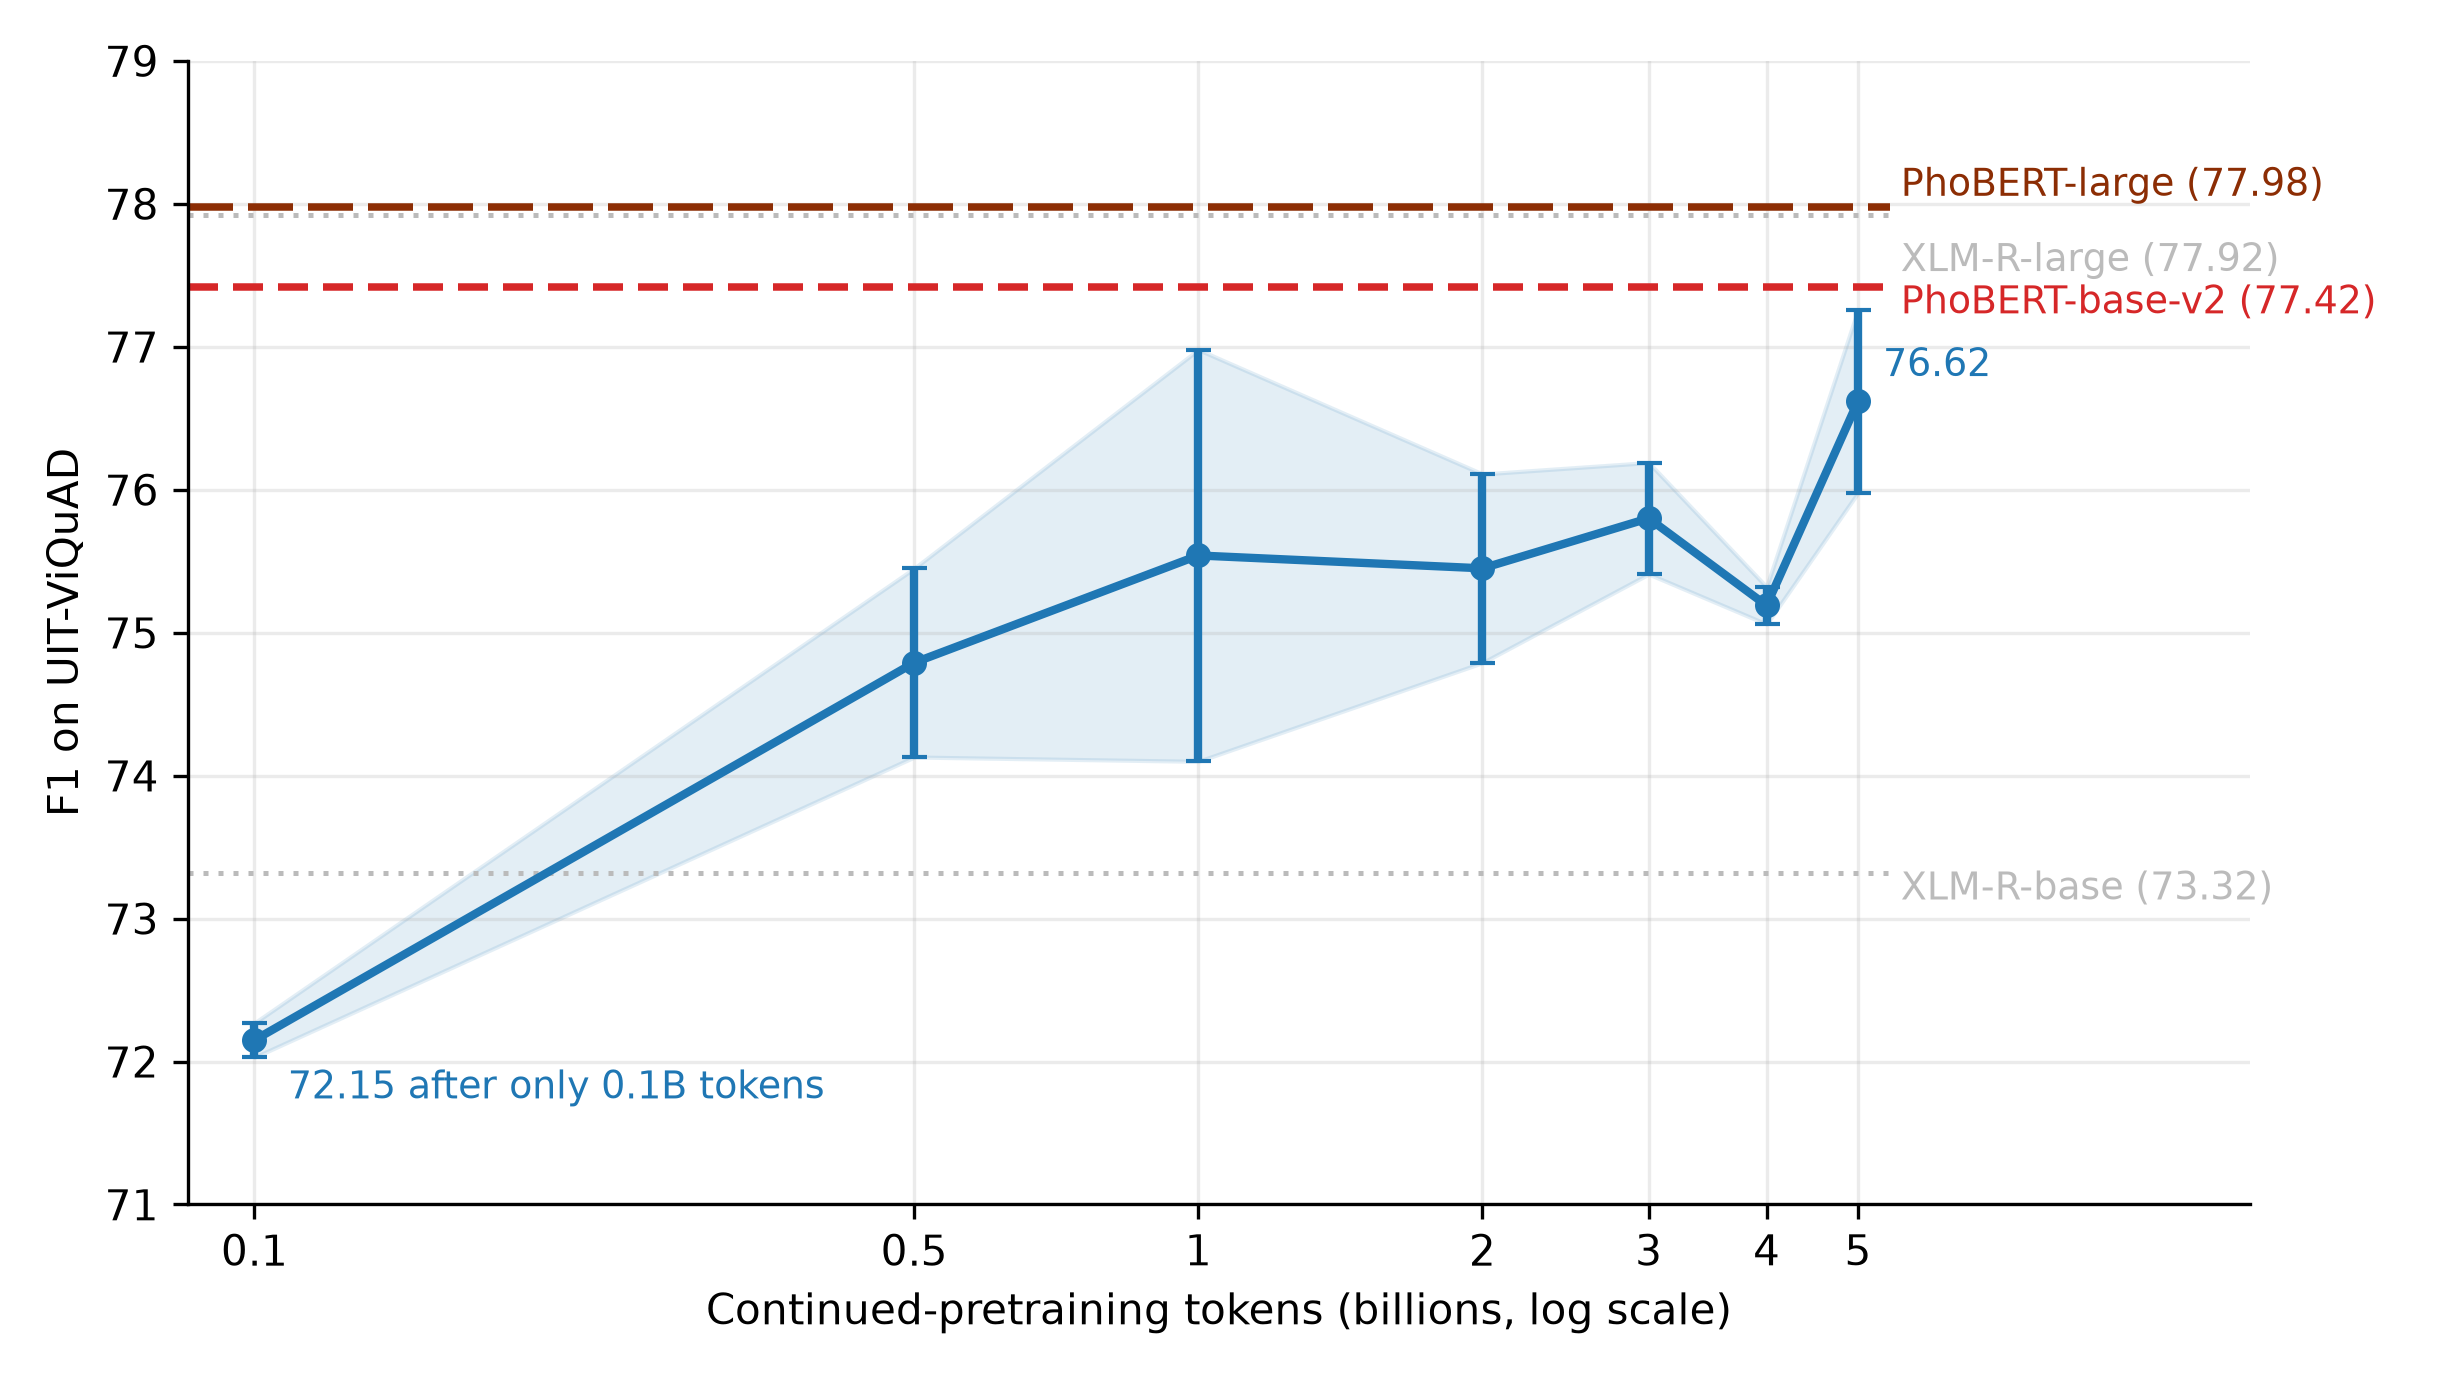
\includegraphics[width=\linewidth]{fig-f1-tokens}\\[2pt]
  {\footnotesize\color{vnCite} Hình: F1 trên UIT-ViQuAD theo số token CPT
   (thang log)}
\end{column}

\begin{column}{0.43\textwidth}
  \small
  \begin{tabular}{@{}l r@{}}
    \toprule
    \rowcolor{vnLight}
    \color{vnNavy}\bfseries Mốc ngân sách &
    \color{vnNavy}\bfseries F1\\
    \midrule
    0,1 tỷ token (2\% ngân sách) & 72,15\\
    0,5 tỷ token                 & 74,79\\
    \ourrow 5 tỷ token (cuối)    & \hl{76,62}\\
    \midrule
    XLM-R-base (cuối)            & 73,32\\
    PhoBERT-base-v2              & 77,4\\
    PhoBERT-large                & 78,0\\
    \bottomrule
  \end{tabular}

  \vspace{0.5em}
  \begin{itemize}\itemsep1pt
    \item Vượt XLM-R-base ngay tại mốc \textbf{0,5 tỷ token}.
    \item Còn cách PhoBERT-base-v2 \textbf{0,8} điểm và PhoBERT-large
          \textbf{1,4} điểm -- xu hướng vẫn đang đi lên.
  \end{itemize}
\end{column}
\end{columns}
\end{frame}

% ---------------------------------------------------------------------
\begin{frame}{Kết quả trên 12 tác vụ hiểu tiếng Việt}
\vspace{0.2em}
\scriptsize
\begin{tabular}{@{}l l r r r r r@{}}
  \toprule
  \rowcolor{vnLight}
  \color{vnNavy}\bfseries Tác vụ & \color{vnNavy}\bfseries Độ đo &
  \color{vnNavy}\bfseries PhoBERT-v2 & \color{vnNavy}\bfseries PhoBERT-L &
  \color{vnNavy}\bfseries XLM-R-B & \color{vnNavy}\bfseries XLM-R-L &
  \color{vnNavy}\bfseries ViNeoBERT\\
  \midrule
  UIT-VSFC        & F1-w        & 0,9345 & \best{0,9356} & 0,9281 & 0,9312 & 0,9284\\
  UIT-VSMEC       & F1-m        & \best{0,6415} & 0,6132 & 0,6145 & 0,3125 & 0,6163\\
  UIT-ViCTSD      & F1-m        & 0,7455 & \best{0,7526} & 0,7110 & 0,5759 & 0,7315\\
  ViCoLA-syn      & MCC         & \best{0,8103} & 0,7915 & 0,7827 & 0,4845 & 0,7789\\
  XNLI (vi)       & Acc         & 0,7720 & 0,7769 & 0,7541 & \best{0,8000} & 0,7714\\
  ViANLI          & F1-m        & \best{0,4529} & 0,3882 & 0,3625 & 0,1666 & 0,4273\\
  QNLI (vi)       & Acc         & 0,8872 & 0,8861 & 0,8592 & \best{0,8940} & 0,8791\\
  \ourrow
  UD-VTB (POS)    & F1-m        & 0,7799 & 0,7879 & 0,7827 & 0,8062 & \best{\color{vnRed}0,8089}\\
  STS (vi)        & Spearman    & 0,8557 & 0,8509 & 0,8226 & \best{0,8644} & 0,8392\\
  Paraphrase      & F1-m        & 0,9351 & 0,9400 & 0,9016 & \best{0,9437} & 0,9276\\
  Retrieval       & nDCG@10     & \best{0,4719} & 0,4659 & 0,1386 & 0,2565 & 0,4061\\
  Reranking       & MRR         & \best{0,8922} & 0,8794 & 0,5282 & 0,6741 & 0,8448\\
  \bottomrule
\end{tabular}

\vspace{0.4em}
\begin{columns}[T]
\begin{column}{0.49\textwidth}
  \footnotesize
  \begin{itemize}\itemsep0pt
    \item Cao hơn XLM-R-base \hl{11/12} tác vụ (12/13 nếu tính đọc hiểu).
    \item \textbf{Dẫn đầu cả bảng} ở gán nhãn từ loại.
  \end{itemize}
\end{column}
\begin{column}{0.49\textwidth}
  \footnotesize
  \begin{itemize}\itemsep0pt
    \item XLM-R-large \emph{bất ổn} rõ rệt trên dữ liệu nhỏ (VSMEC 0,31;
          ViANLI 0,17); ViNeoBERT ổn định trên cả 12 tác vụ.
    \item Điểm mạnh tập trung ở biểu diễn \emph{cấp token} -- đúng năng lực
          kế thừa từ phần thân 28 lớp.
  \end{itemize}
\end{column}
\end{columns}
\end{frame}

% ---------------------------------------------------------------------
\begin{frame}{Luận điểm trung tâm: hiệu quả dữ liệu}
\vspace{0.3em}
\begin{columns}[T]
\begin{column}{0.55\textwidth}
  \small
  \begin{tabular}{@{}l r r@{}}
    \toprule
    \rowcolor{vnLight}
    \color{vnNavy}\bfseries Mô hình &
    \color{vnNavy}\bfseries Token tiếng Việt &
    \color{vnNavy}\bfseries F1 ViQuAD\\
    \midrule
    PhoBERT-large   & $\sim$140 tỷ (40 lượt) & 78,0\\
    PhoBERT-base-v2 & $>$140 tỷ              & 77,4\\
    XLM-R-base      & hàng trăm tỷ           & 73,3\\
    \ourrow
    \textbf{ViNeoBERT} & \hl{5 tỷ (1 lượt)}  & \textbf{76,6}\\
    \bottomrule
  \end{tabular}

  \vspace{0.6em}
  \fitpic{\begin{tikzpicture}[font=\scriptsize,x=1cm,y=0.42cm]
    \fill[vnNavy!25] (0,0) rectangle (7.8,0.8);
    \fill[vnRed]     (0,0) rectangle (0.273,0.8);
    \node[right,text=vnNavy,font=\tiny] at (0.4,0.4)
         {PhoBERT-large: $\sim$140 tỷ token};
    \node[text=vnRed,font=\tiny,anchor=north west] at (0,-0.15)
         {ViNeoBERT: 5 tỷ (3,5\%)};
  \end{tikzpicture}}
\end{column}

\begin{column}{0.43\textwidth}
  \begin{block}{Con số đáng nói nhất}
    \small Với \hl{3,5\%} lượng token mà PhoBERT-large đã huấn luyện,
    ViNeoBERT đạt \textbf{98,3\%} điểm F1 của mô hình đó -- dù
    PhoBERT-large lớn gấp 1,5 lần về tham số.
  \end{block}

  \vspace{0.3em}
  \begin{itemize}\itemsep1pt
    \item Xác nhận trực tiếp giả thuyết của khóa luận: \emph{tái sử dụng}
          không gian biểu diễn cho phép kế thừa năng lực phần thân thay vì
          học lại từ đầu.
    \item Có ý nghĩa đặc biệt với các ngôn ngữ ít tài nguyên.
  \end{itemize}
\end{column}
\end{columns}
\end{frame}

% ---------------------------------------------------------------------
\begin{frame}{Biến trần 4.096 token thành năng lực dùng được}
\vspace{0.2em}
\begin{columns}[T]
\begin{column}{0.57\textwidth}
  \centering
  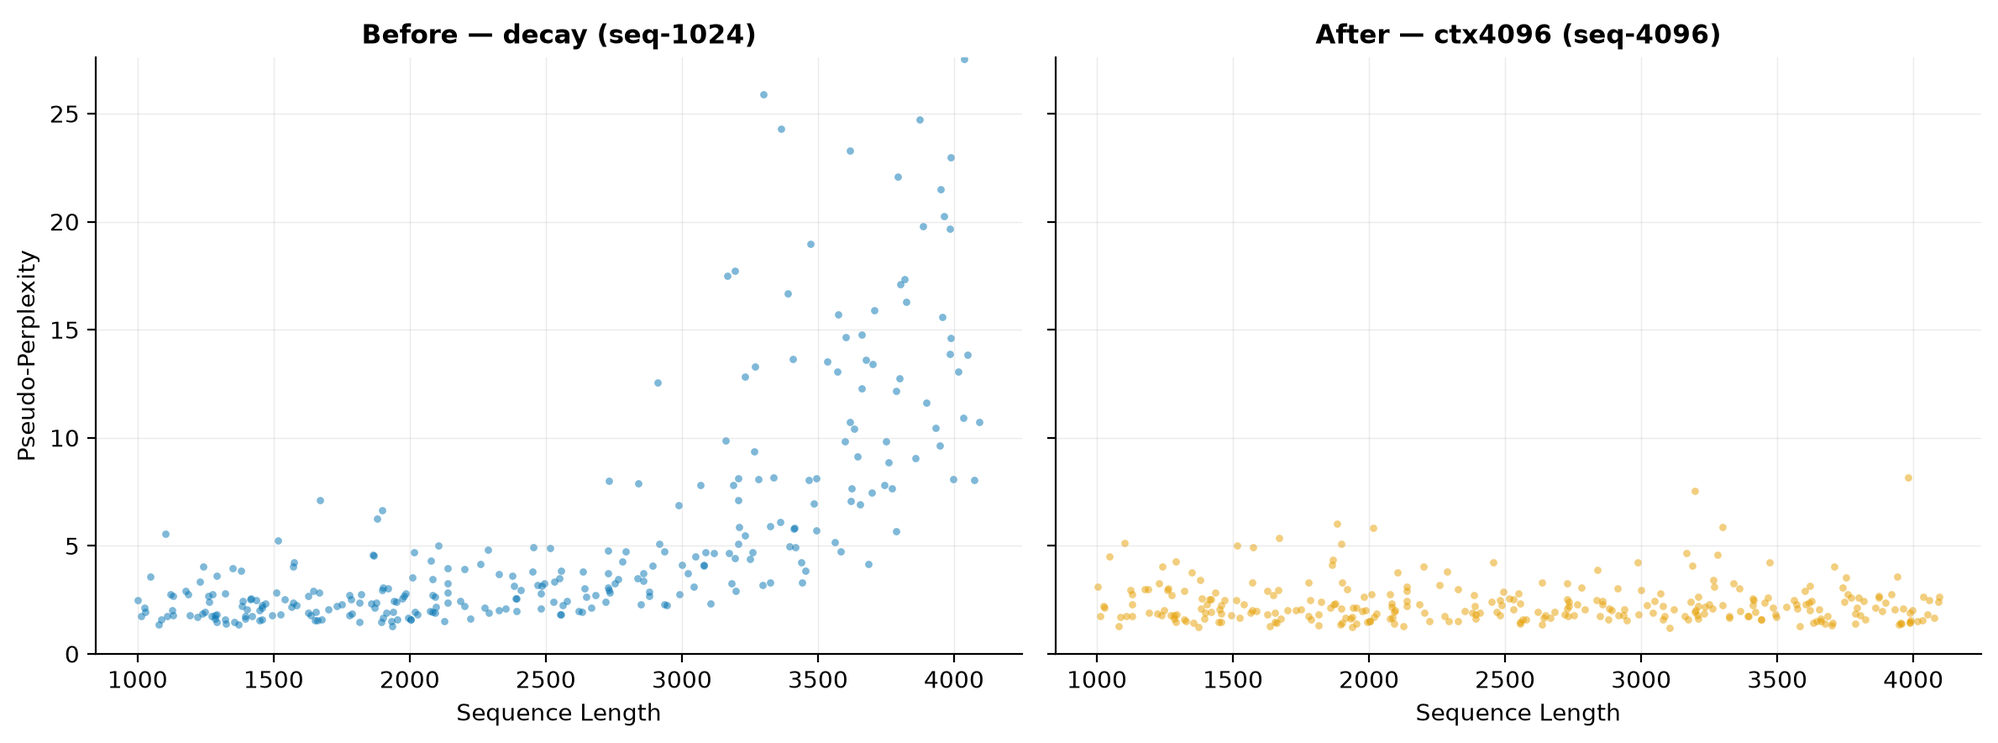
\includegraphics[width=\linewidth]{fig-pppl-ctx}\\[2pt]
  {\footnotesize\color{vnCite} Hình: pseudo-perplexity theo độ dài chuỗi,
   trước và sau pha mở rộng ngữ cảnh}
\end{column}

\begin{column}{0.41\textwidth}
  \small
  Toàn bộ CPT chạy ở độ dài 1.024 token. Sau đó huấn luyện thêm
  \textbf{$\sim$200 triệu token} ($\sim$4\% ngân sách) ở độ dài 4.096.

  \vspace{0.5em}
  \begin{itemize}\itemsep2pt
    \item \textbf{Trước}: nhờ tính tương đối của RoPE, mô hình ngoại suy ổn
          định tới $\approx$2.500--3.000 token, sau đó chất lượng
          \emph{giảm nhanh} (nhiều điểm vượt 10).
    \item \textbf{Sau}: pseudo-perplexity phẳng quanh \hl{2--3} trên toàn dải
          tới 4.096 token.
  \end{itemize}

  \vspace{0.3em}
  {\footnotesize\color{vnCite} Đo theo đúng giao thức của NeoBERT
   \citep{Salazar2020}.}
\end{column}
\end{columns}
\end{frame}

% =====================================================================
\section{Kết luận và hướng phát triển}
% =====================================================================

% ---------------------------------------------------------------------
\begin{frame}{Kết luận}
\vspace{0.3em}
\begin{columns}[T]
\begin{column}{0.49\textwidth}
  \textbf{Đóng góp của khóa luận}
  \begin{itemize}\itemsep2pt
    \item \textbf{ViNeoBERT} -- Encoder hiện đại $\approx$250 triệu tham số
          cho tiếng Việt, kế thừa RoPE/SwiGLU/Pre-RMSNorm và trần ngữ cảnh
          4.096 token.
    \item \textbf{Quy trình chuyển đổi ngôn ngữ} ba giai đoạn, lần đầu áp
          dụng cho một kiến trúc Encoder thế hệ mới.
    \item \textbf{Ba cải tiến so với SALT gốc}: điểm neo theo cặp dịch,
          khởi tạo riêng lớp đầu ra, giai đoạn căn chỉnh với thân đóng băng.
    \item \textbf{Bộ mã nguồn công khai} cùng toàn bộ kịch bản huấn luyện.
  \end{itemize}
\end{column}

\begin{column}{0.49\textwidth}
  \textbf{Kết quả chính}
  \begin{itemize}\itemsep2pt
    \item \hl{76,62} điểm F1 trên UIT-ViQuAD -- hơn XLM-R-base 3,3 điểm.
    \item Cao hơn XLM-R-base ở \textbf{11/12} tác vụ; dẫn đầu cả bảng ở gán
          nhãn từ loại.
    \item Từng lựa chọn thiết kế đều được kiểm chứng có kiểm soát:
          $\gamma=0{,}1$, khởi tạo riêng hai ma trận (67,52 so với 54,09),
          căn chỉnh với thân đóng băng ($-26\%$ perplexity).
    \item Ngữ cảnh 4.096 token trở thành năng lực dùng được với chỉ
          $\sim$200 triệu token bổ sung.
    \item[$\Rightarrow$] Tất cả đạt được với \hl{3,5\%} lượng token của
          PhoBERT-large.
  \end{itemize}
\end{column}
\end{columns}
\end{frame}

% ---------------------------------------------------------------------
\begin{frame}{Hạn chế và hướng phát triển}
\vspace{0.3em}
\begin{columns}[T]
\begin{column}{0.47\textwidth}
  \textbf{Hạn chế}
  \begin{itemize}\itemsep2pt
    \item \textbf{Ngân sách huấn luyện}: 5 tỷ token vẫn nhỏ; chưa vượt
          PhoBERT-base-v2 ở nhóm phân loại câu ngắn.
    \item \textbf{Phạm vi đánh giá}: chưa khảo sát nhận dạng thực thể có tên.
    \item \textbf{Ngữ cảnh dài}: mới kiểm chứng bằng độ đo nội tại
          (pseudo-perplexity), chưa có tác vụ ứng dụng.
    \item \textbf{Tokenizer}: kế thừa ViDeBERTa, chạy ở mức âm tiết trên văn
          bản thô -- \emph{không tách từ} như PhoBERT; ảnh hưởng của khác
          biệt này chưa được phân tích riêng.
  \end{itemize}
\end{column}

\begin{column}{0.50\textwidth}
  \textbf{Hướng phát triển}
  \begin{enumerate}\itemsep2pt
    \item \textbf{Mở rộng ngân sách CPT} -- đường cong F1 vẫn đang đi lên.
    \item \textbf{Trộn lại 5--10\% dữ liệu tiếng Anh} như cơ chế phát lại
          (replay) để giảm mất thông tin \cit{Elhady2025}.
    \item \textbf{Đánh giá trên tác vụ ngữ cảnh dài} (hỏi đáp đa đoạn, truy
          xuất tài liệu); vượt trần 4.096 token bằng YaRN \cit{Peng2023}.
    \item \textbf{Mở rộng bộ đánh giá} -- NER, truy xuất quy mô lớn, lặp lại
          nhóm biểu diễn câu qua nhiều seed.
    \item \textbf{Tổng quát hóa quy trình} sang ngôn ngữ ít tài nguyên khác
          và kiến trúc nền khác.
  \end{enumerate}
\end{column}
\end{columns}
\end{frame}

% ---------------------------------------------------------------------
\begin{frame}[plain]
  \vfill
  \centering
  {\color{vnSteel!45}\rule{0.55\textwidth}{0.8pt}\par}
  \vspace{0.7em}
  {\Large\bfseries\color{vnNavy} Xin chân thành cảm ơn quý thầy cô\\[4pt]
   đã lắng nghe phần trình bày.\par}
  \vspace{0.7em}
  {\color{vnSteel!45}\rule{0.55\textwidth}{0.8pt}\par}

  \vspace{1.2em}
  {\small\color{vnCite} Nhóm rất mong nhận được các ý kiến đóng góp của hội đồng.\par}
  \vfill
\end{frame}

% =====================================================================
\section*{Tài liệu tham khảo}
% =====================================================================
\begin{frame}[allowframebreaks]{Tài liệu tham khảo}
  \scriptsize
  % Slide giữ tối thiểu trích dẫn để đỡ rối; \nocite{*} đưa toàn bộ refs.bib vào
  % danh mục nên tài liệu tham khảo vẫn đầy đủ dù không được trích dẫn trên slide.
  \nocite{*}
  \bibliographystyle{apalike}
  \bibliography{refs}
\end{frame}


\end{document}
